
\Chapter{\label{CH:challenges}Challenges in data reduction}{Etalon cavity map}

Thus far, we have focused on TuMag, its properties, and the correction of its data due to its central role in this thesis. However, there are other tunable spectropolarimeters, each with its own specific characteristics, advantages, and challenges. In this chapter, we shift our focus away from TuMag and turn our attention to another class of magnetographs, specifically those with their etalon in a telecentric configuration.

Currently, there is an ongoing debate within the scientific community regarding the optimal optical configuration for the etalon in spectropolarimeters, whether it should be collimated or telecentric. This debate has garnered significant interest, as evidenced by the numerous studies addressing the properties of each configuration. Notable contributions include the four works by Bailén et al. (\citealt{franI}, \citealt{franII}, \citealt{franIII}, \citealt{franIV}), an extensive analysis on topics such as the impact of defects, applications for instrumentation, and the analytical formulation of the etalon's transmission profiles. Other examples include the studies by \citep{beckers} and \citep{ghosts-etalon}, which analyze the optical performance of FPIs, as well as the works of \citealt{kentischer1998tesos} and \citealt{cavallini2006ibis}, which discuss the properties of the etalons in the Telecentric Etalon Solar Spectropolarimeter (TESOS) and the Interferometric BIdimensional Spectrometer (IBIS), respectively. Additionally, the review of \citealt{fran_review} provides a broad and comprehensive overview of this topic. The reality is that it is challenging to provide a definitive answer to this question, as each configuration has its own advantages and disadvantages.

The primary argument against collimated mounts is the amplification of wavefront errors resulting from the large footprint of the light rays on the etalon plates, which includes both large and small scale defects \citep{fran_review}. This amplification deteriorates the optical quality of these setups and has promoted the use of telecentric setups, where the footprints of the light rays are much smaller and the optical performance is less affected by large scale defects.

Despite its potential benefits, the telecentric configuration is no exempt of challenges. In this configuration each light ray trasverses the etalon through different regions, thus being affected differently at each point from the various small scale defects present in the etalon. This defects, compose the so-called, cavity-map and its correction can be one of the main challenges of employing this setups.

This chapter aims to provide a comprehensive examination of telecentric configurations for etalons within the context of solar spectropolarimeters. We will begin by exploring the analytical formulation of the transmission profiles and spatial PSF of FPI's in both collimated and telecentric configurations. Following this, we will delve into the effects of the cavity error in solar observations, through a simulation of an observation of a Sunspot. Then, we will present a strategy to derive the cavity map from flat field observations in an attempt to improve the data correction. This strategy is presented and tested in a forthcoming academic paper under the title of "Correcting Fabry-Perot etalon effects in solar observations" \footnote{DOI :  https://doi.org/10.1051/0004-6361/202449825}, and the contents of the corresponding section will be extracted from there. 

\section{One device, two configurations.}

We established in section \ref{susec_spectropolarimeters: Imaging} that the observed intensity distribution at the coordinates $\xi$, $\eta$ of the focal plane of any etalon-based instrument tuned to a wavelength $\lambda_s$ obeys the following expression \citep{franI}: 

\begin{equation}
    I\left(\xi, \eta ; \lambda_{s}\right)=g(\xi, \eta)\int_{0}^{\infty} T(\lambda) \iint  O\left(\xi_0, \eta_0 ; \lambda\right)  \mathcal{S}\left(\xi_0, \eta_0; \xi , \eta; \lambda-\lambda_{s}\right)  \mathrm{d} \xi_{0} \mathrm{~d} \eta_{0}\mathrm{d} \lambda ,
    \label{eq_etalon_theory: General_Intensity}
\end{equation}
where $T(\lambda)$ accounts for the presence of an order-sorting pre-filter, $O\left(\xi_0, \eta_0 ; \lambda\right)$ represents the brightness distribution of the observed object at the point $\left(\xi_0, \eta_0\right)$, $S\left(\xi_0, \eta_0; \xi , \eta; \lambda-\lambda_{s}\right)$ accounts for the imaging response of the instrument when tuned at the wavelength $\lambda_{s}$, and $g(\xi, \eta)$ represents a spatial gain factor that accounts for wavelength independent pixel-to-pixel intensity fluctuations ocurring in the focal plane due to differences in the detectors' sensitivity. 

The imaging response of the instrument coincides with the PSF of the instrument when the optical response is invariant against translations. In such a case, we can substitute the last two integrals by the convolution operator, but this is not strictly true in etalon-based instruments, where the response varies pixel to pixel either because of etalon irregularities or because of variations in the illumination across its clear aperture.

Deriving S typically requires determining the electric field of the polychromatic wave in the image plane. According to \cite{franI}, this field can be calculated by summing all the electric fields $(E^{(t)})$ across the pupil, such that the eletric field at any point $(\xi, \eta)$ of the image plane follows the expression:

\begin{equation}
  E_{im} ^{(t)}(\xi, \eta) = \frac{1}{\pi R_{pup} ^2} \int \int _ {pupil} E^{(t)}(x, y)e ^{-ik( \xi x / f + \eta y / f)dx dy},
  \label{eq_etalon_theory: electric_image_plane}
\end{equation}
where $(x, y)$ are the coordinates in the pupil, $f$ stands for the focal length, and $R_{pup}$ is the radius of the pupil.  It can also be shown that the vector electric fields transmitted by the etalon can be expressed as:

\begin{equation}
  E ^{(t)}(\xi, \eta) = \frac{\sqrt{\tau}}{1 - R}\frac{e ^{i\delta / 2} - R e ^{ -i\delta / 2}}{1 + F \sin ^2 (\delta / 2)}E ^{(i)},
  \label{eq_etalon_theory: electric_transmitted}
\end{equation}
where $\tau$ is the transmission factor for normal incidence, $R$ stands for the reflectivity of the etalon mirrors, $F$ is a factor defined as $F \equiv 4R (1 - R )^{-2}$, $E^{(i)}$ are the incident electric fields, and $\delta$ stands for the phase differences between the transmitted and incident rays. 

The transmission profile of the etalon ($S$) is defined as the average ratio between the transmitted and incident intensities, calculated from the complex conjugate of the corresponding electric fields. The shape of $\delta$ varies depending on the illumination setup of the etalon, whether collimated or telecentric. Consequently, each configuration has unique solutions and characteristics and is differently affected by inhomogeneities (defects) in the etalon's properties.

\subsection{\label{susec_etalon_theory: collimated}Collimated configuration}

\begin{figure}
  \centering
  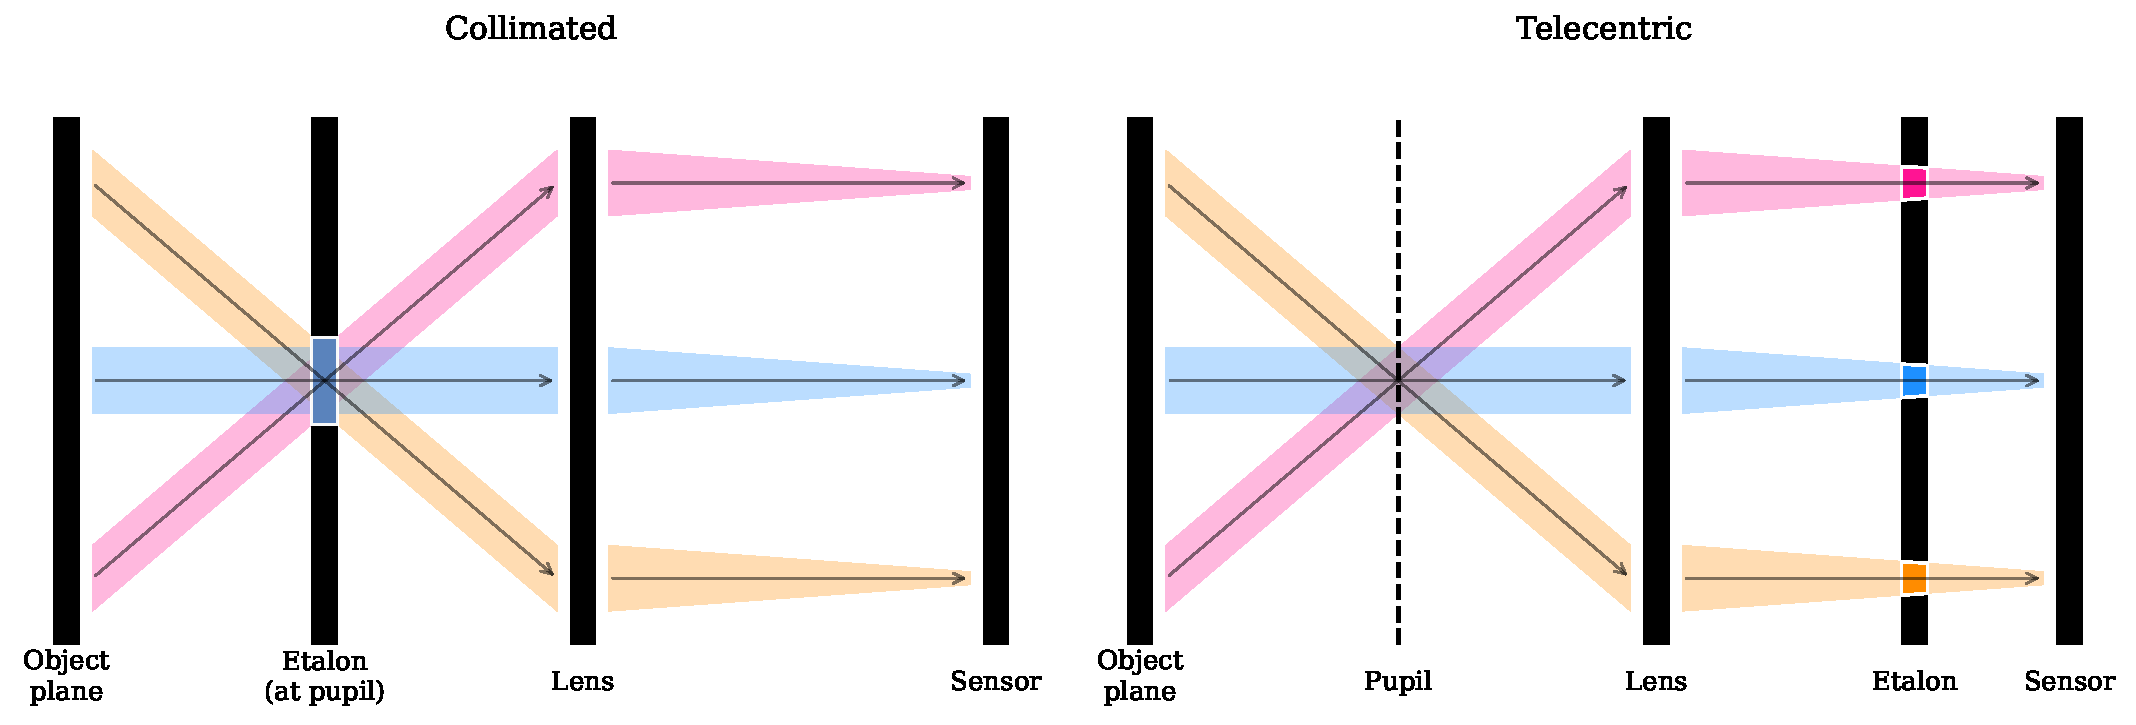
\includegraphics[width = \textwidth]{figures/EtalonChallenges/EtalonConfigurations.pdf}
  \caption{Schematic representation of the two optical setups of an FPI, collimated (left) and telecentric (right). The different colors represent distinct light rays originating from various points on the object plane. The white boxes in the etalon highlight the sections that are traversed by the light rays.
  } \label{fig_etalon_theory: Etalon configurations}
\end{figure}

Collimated mounts are characterized by having the etalon located at the pupil plane and therefore receive a collimated beam from each point of the observed object. As illustrated in the schematic on the left side of fig.~{\ref{fig_etalon_theory: Etalon configurations}}, light from any point on the object will fall on the same area of the etalon. Consequently, any local defects on the etalon crystals or on the plates' parallelism is averaged all over the clear aperture, thus making the optical quality constant along the FoV. However, the angle of incidence of the light beam varies along the FoV, thus shifting the spectral transmission profile.  

Analytical solutions of equation \eqref{eq_etalon_theory: electric_image_plane} are imposible to obtain if $\delta$ has a dependence on the pupil coordinates, as is the case of collimated etalons with a presence of local defects. In that case, the transmssion profile of the etalon has to be evaluated numerically. 

However, in order to study the spectral behavior of the transmission profile, we can, as a first-order approximation, disregard the spatial PSF and focus solely on the spectral transmission profile $(\psi)$. Under this assumption, the phase difference between the incident and transmitted rays of an ideal collimated etalon can be expressed as:  

\begin{equation}
  \delta (\xi, \eta, \lambda) = \frac{4\pi}{\lambda}nd\cos (\theta(\xi, \eta)),
  \label{eq_etalon_theory: collimated_delta}
\end{equation}
where $n$ stands for the refractive index of the etalon cavity, $d$ is the distance between the mirrors and $\theta$ is the angle of incidence. In such a case, it can be shown that the spectral transmission profile follows the expression: 

\begin{equation}
  \psi\left(\xi, \eta, \lambda \right) = \frac{\tau}{1 + F \sin ^2 (\delta(\xi, \eta, \lambda) / 2)}.
  \label{eq_eta_theory : Collimated_profile}
\end{equation}

The spectral behaviour of the transmission profile, such as the spectral position of the resonance peaks and the distance between them (the free spectral range), is encoded in the parameter $\delta$, which is a function of the refractive index of the etalon cavity, the distance between mirrors, and the angle of the incident beam. The reflectivity $R$ of the mirrors determines the width of the resonance peaks through the parameter $F$, $F \equiv 4R (1 - R )^{-2}$.

Local defects in the collimated configuration are averaged out, which means that $d$ and $n$ respectively represent the mean values of the thickness and refractive index across the clear aperture of the FPI, and thus remain constant for every pixel. Yet, they produce a broadening of the transmission profile and worsen the optical quality of the instrument. However, the spatial dependence of $\psi$ naturally arises from $\theta$, which vcaries from pixel to pixel. 

Assessing the spatial PSF of the FPI is more challenging, as it can only be determined analytically for monochromatic light and in the absence of defects. We will not delve into the equations for this specific scenario as it lies beyond the scope of this thesis. However, interested readers are referred to the work of \cite{franI}, where this topic is extensively discussed.

\subsection{\label{susec_etalon_theory: Tele-perfe}Telecentric configuration}

In the telecentric configuration, the etalon is placed very close to an intermediate focal plane, while the pupil is focused at infinity. As shown in the sketch on the right side of fig.~{\ref{fig_etalon_theory: Etalon configurations}}, in this setup, the etalon is illuminated by cones of rays that are parallel to each other, thus passing through different sections of the interferometer. Local inhomogeneities (defects or cavities) on the etalon produce differences in the transmission profile across the FoV, which are directly mapped into the image plane. This means that the optical response and the transmission profile shift locally on the image sensor. 

In telecentric configurations, $\delta$ always depends on the coordinates of the pupil, even in the absence of defects, since each point in the etalon sees a cone of rays coming from different parts of the pupil. Thus, as stated before, solutions to equation \eqref{eq_etalon_theory: electric_image_plane} are to be found numerically. Nonetheless, if we neglect the spatial PSF once again, we can derive an analytical expression for an ideal telecentric etalon, where all light cones impact perpendicularly.

After some messy algebra and clever variable changes, one can recast eq. \eqref{eq_etalon_theory: electric_image_plane} in terms of the radial coordinates of the pupil and anallytically solve the equations. The resulting spectral transmission profile of an ideal telecentric etalon  is given by \citep{franIV}:
\begin{equation}
\Psi \left(\xi, \eta, \lambda \right) =  \mathfrak{Re}\left[E(a\left(\xi, \eta, \lambda \right), b\left(\xi, \eta, \lambda \right)) \right] ^2 + \mathfrak{Im}\left[E(a\left(\xi, \eta, \lambda \right), b\left(\xi, \eta, \lambda \right)) \right] ^2 ,
\label{eq_etalon_theory: Tel_first}
\end{equation}
with $E(a\left(\xi, \eta, \lambda \right), b\left(\xi, \eta \right))$ being:
\begin{multline}
E(a\left(\xi, \eta, \lambda \right), b\left(\xi, \eta \right)) = 2\sqrt{\tau}\Biggl\{ \frac{1}{\alpha_1}\left[\arctan(\gamma _ 1) - \arctan(\gamma_2)\right] + \\
\mathrm{i} \frac{1+R}{1-R} \frac{1}{\alpha_2}\left[\ln \left(\frac{(1 + \gamma _ 3) ^2 + \gamma _ 4 ^2}{(1 - \gamma _ 3) ^2 + \gamma _ 4 ^2} \right) - \ln \left(\frac{(1 + \gamma_ 3) ^2 + \gamma _ 5 ^ 2}{(1 - \gamma _ 3) ^2 + \gamma _ 5 ^2} \right)\right]\Biggr\},  
\end{multline}
where, the auxiliary functions are defined as:
\begin{equation}
\begin{split}
a\left(\xi, \eta, \lambda \right) &\equiv \frac{2 \pi}{\lambda}n\left(\xi, \eta\right)d\left(\xi, \eta\right) \ , \\
b\left(\xi, \eta\right) &\equiv \frac{1}{8n\left(\xi, \eta\right)^2(f\#) ^2}\ ,  \\
\alpha _ 1 &\equiv 2ab\sqrt{F}\ ,  \\
\alpha _ 2 &\equiv 2\alpha_ 1\sqrt{F + 1}\ ,  \\
\gamma _ 1 &\equiv \sqrt{F} \sin a\ ,  \\
\gamma _ 2 &\equiv \sqrt{F} \sin (a[1 - b])\ ,  \\
\gamma _ 3 &\equiv \sqrt{\frac{F}{F + 1}} \ ,  \\
\gamma _ 4 &\equiv \frac{\tan \left( a/2 [1 - b] \right)}{\sqrt{F + 1}}\ ,  \\
\gamma _ 5 &\equiv \frac{\tan (a/2)}{\sqrt{F + 1}}\ .
\end{split}
\end{equation}

The parameter $a$ has the same role as $\delta$ for the collimated case. However, the dependence on the image plane coordinates in this case is caused by potential variations in n and/or d, as each light beam traverses different sections of the etalon. These variations constitute the "cavity map" of a telecentric etalon and must always be taken into account during data reduction processes.

The parameter $b$ accounts for the contribution of the focal ratio, $f\#$, and has an impact on the spectral resolution and the apodization of the pupil as seen from the etalon \citep{beckers}. Thus, the resolution is now affected by both $F$ and $f\#$, through the parameters $a$ and $b$.

\subsubsection{\label{etalon_theory: Tele-imperfe}Telecentric imperfect configuration}
The equations shown in Sect.~\ref{susec_etalon_theory: Tele-perfe} are valid whenever the incident cone of rays is perpendicular to the etalon mirrors. We refer to this situation hereinafter as "perfect telecentrism". However, real instruments are likely to present deviations from such an ideal case. These deviations can be caused by an intentional tilt of the etalon to suppress ghost images on the detector \citep{ghosts-etalon}, by an accidental tilted angle of incidence caused by deviations from the ideal paraxial propagation of rays within the instrument, or simply because of misalignment of the optical components. In the three cases, the incident cone of rays is no longer perpendicular to the etalon, and hence, we consider these scenarios to have imperfections in the telecentrism degree. One important consequence of the loss of telecentrism is an asymmetrization of the transmission profile that must be accounted for when modeling the instrument response.

The transmission profile in this case is influenced by the angle of incidence of the chief ray at each point of the clear aperture of the etalon, in addition to the parameters mentioned in the previous sections. Unfortunately, the equations for the transmission profile in these configurations are much more complicated than in the ideal case, and can no longer be anallytically solved. We must revisit equation \eqref{eq_etalon_theory: electric_image_plane} and solve the integrals numerically.

\begin{figure}
    \centering
    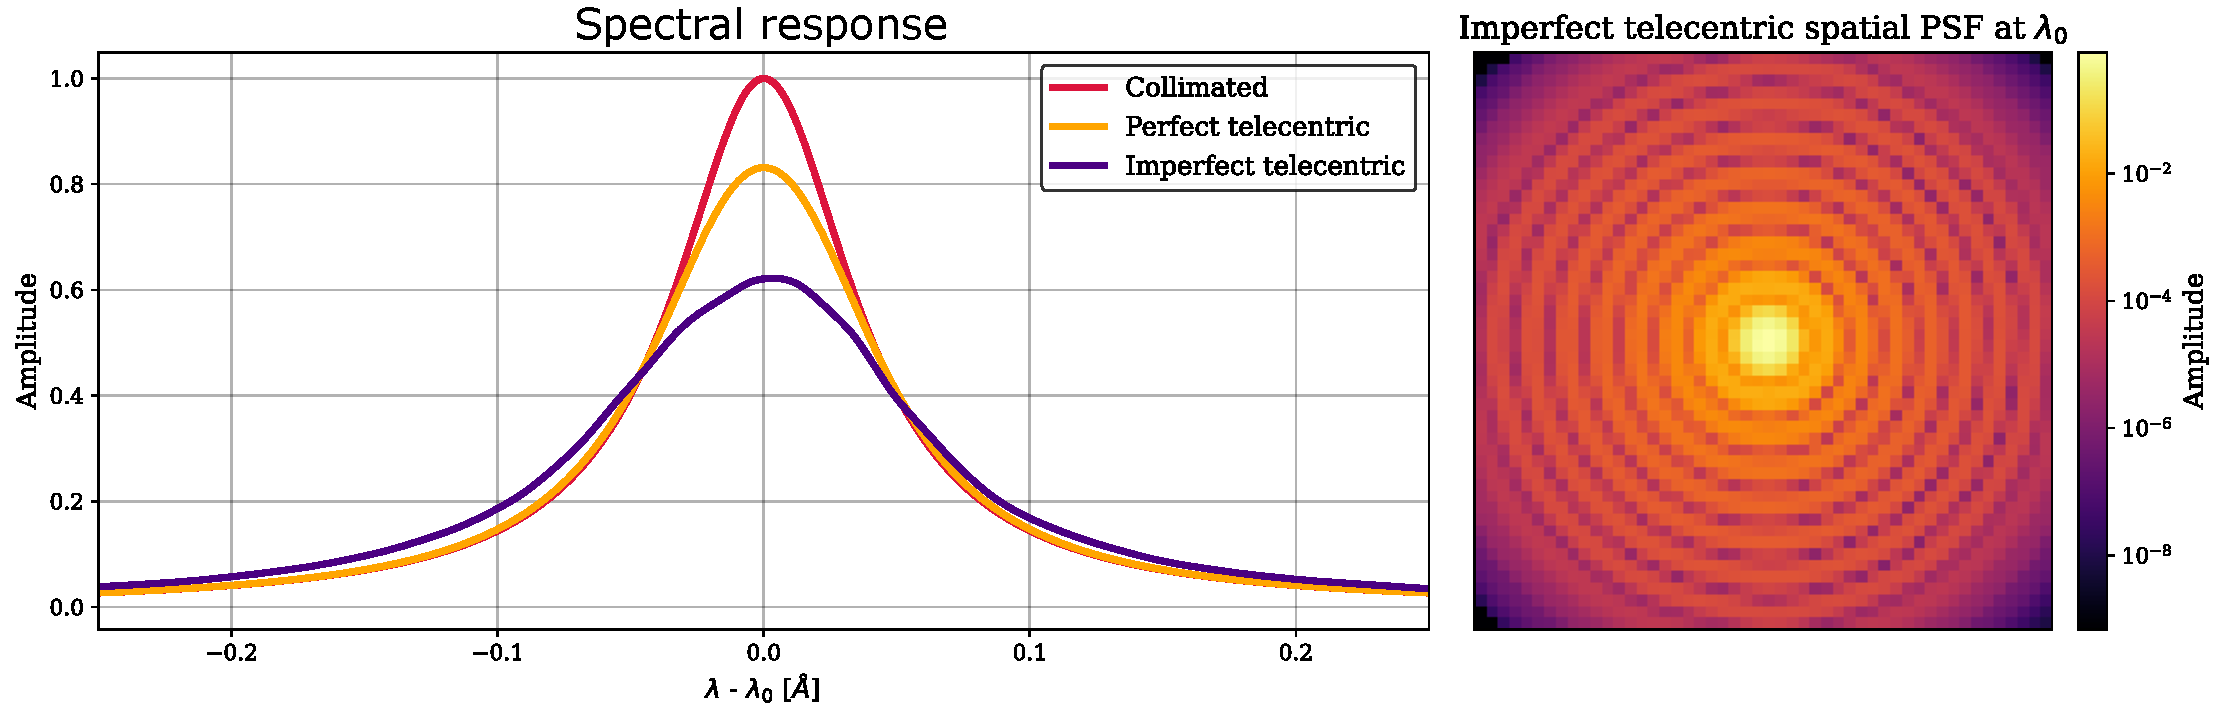
\includegraphics[width = \textwidth]{figures/EtalonChallenges/etalon_setups_profiles.pdf}
    \caption{\textit{Left}: central peak of the etalon's spectral transmission profile for the three different configurations. \textit{Right}: Spatial PSF of the imperfect telecentric etalon at $\lambda _ 0$. The parameters of the etalon are $R = 0.92$, $n = 2.29$, $d = 251 \, \mu \mathrm{m}$, $f\#=56$, $\theta = 0 ^{\circ}$ (collimated and perfect telecentric), and $\Theta = 0.3\,^{\circ}$ (imperfect telecentric).}
    \label{fig_etalon_theory:Profiles-configs}
\end{figure}

Figure \ref{fig_etalon_theory:Profiles-configs} shows on the left the transmission profile corresponding to the three different scenarios: collimated illumination of the etalon, perfect telecentrism, and imperfect telecentrism. The etalon parameters have been selected to coincide with those of SO/PHI's etalon. In both the collimated and perfect telecentric configurations, a normal incidence  ($\theta = 0$) scenario is shown, whereas in the imperfect telecentric case, we assumed an angle of incidence of the chief ray, $\Theta$, of $0.3^{\circ}$. The parameter $a$ has been adjusted slightly in order to tune the transmission profile at $\lambda _ 0$. 

Regarding the properties of each profile, note that the telecentric configurations achieve lower peak transmissions than the collimated case. In addition, the telecentric profiles are wider due to the different incidence angles across the illuminating cone of rays. Such a broadening increases with decreasing f-ratios. Lastly, non-normal incidence of the chief ray in the telecentric configuration further widens and shifts ($\sim 4$~m\r{A}
for $\Theta=0.3^\circ$) the profile, making it asymmetrical. 

\section{\label{sect: Mancha_obs}Sunspot observation simulation}

The analytical formulations equip us with the tools necessary to investigate the impact of the cavity map on observational data and the consequences of incorrect or incomplete corrections. To this end, we will simulate a series of observations of a sunspot using a telecentric FPI and attempt to correct the observations utilizing generated flat-fields. Our aim is to quantify the spurious effects of the cavity map on scientific products, specifically the line-of-sight (LOS) velocities and magnetic field strength.

We have chosen to employ a sunspot for this study since they are one of our main \textit{laboratories} for the study of the magnetic field and dynamics of the solar photosphere. Sunspots are dark regions of the solar surface where strong magnetic fields gather. The innermost part of the spot, the umbra, with a brightness around the 20$\%$ of its surroundings, hosts very strong magnetic fields oriented almost perpendicular to the solar's surface. Surrounding the umbra in fully developed sunspots is the penumbra, a brighter region characterized by a radial filamentary structure with a nearly horizontal outflow of the plasma known as the Evershed flow \citep{evershed}.

The physical mechanisms driving the phenomena in these regions are not yet fully understood and have been a topic of discussion for many years, and still are. Processes such as the Evershed flow lack a universally accepted theoretical model, and numerous studies attempt to provide a theoretical basis for the observations, often presenting conflicting interpretations. Some examples of these works are \citep{evershed_magnetic_flux}, or \citep{evershed_magnetic_2}, where they interpret the evershed flow as a hot gas confinded to magnetic flux tubes that rise due to convecion processes. In contrast, alternative models such as the one proposed by \citealt{evershed_model_scharmer} and \citealt{evershed_model_spruit}, and later updated in \citealt{evershed_magnetic_scharmer}, suggest that the observed filaments are field-free gaps where standard convection occurs. According to these models, the convective cells are elongated as the upward flow is redirected by the inclined magnetic field characteristic of the penumbra, resulting in the outward flow.  

Accurate measurements of velocities and magnetic fields are of paramount importance for deciphering these processes, as the weak and small-scale manifestations of these effects may be crucial for their understanding. Examples for this are the works of \citealt{lateral_downflows_2} or \citealt{lateral_downflows}, where they found and study lateral downflows at the edge of penumbral filaments, supporting the model of penumbral convection from filament dynamics. However, these downflows are very challenging to detect, and require very high spatial resolution and accurate velocity measurements. For this reason, we will focus on the study of the spurious effects of the cavity error in the measurements of velocities and magnetic fields, with a special emphasis on penumbral flows. 

The target of our observations will be a Magnetohydrodynamic (MHD) simulation of a sunspot in the photosphere. We will observe it through the eyes of a telescope of \textcolor{red}{XX meters of aperture} and an FPI similar to the one flying aboard the SO as part of the PHI instrument. This section begins with an overview of the simulated data (Sect.\ref{sect: mancha_sim_data}), followed by a detailed explanation of the observation simulation (Sect.\ref{sect: mancha_obs_sim}). Subsequently, we present and discuss the different flat-fielding strategies in section \ref{sect: mancha_ff_corr}. The section conludes with the discussion of the measurments of the LOS velocities and magnetic field strength in sections \ref{sect: mancha_vlos} and \ref{sect: mancha_blos}, respectively.  


\subsection{\label{sect: mancha_sim_data}Simulated data.}

MHD? From where.  

In order to obtain the magnetic field, we first need to simulate a modulation-demodulation scheme as the ones employed in spectropolarimeters like TuMag or SO/PHI. For this purpose, four different modulations have been generated with etc. 

\subsection{\label{sect: mancha_obs_sim}Observations simulation.}

All the instruments built around the use of an etalon as a wavelength filtering element operate in a very similar way. They scan a spectral line by tuning the etalon (by changing the distance between mirrors and/or modifying the refractive index) to a desired number of wavelengths along the spectral line. At each spectral position, the solar scene is recorded. The measured intensity is approximately given by Eq.~\eqref{eq_etalon_theory: General_Intensity}, with the etalon's transmission profile centered at the desired wavelength.

We have carried out two sets of simulations, one with a perfect telecentric configuration, where the incidence is normal, and one with an angle of incidence of the chief ray is $0.5^\circ$. For each of these sets, a simulated observation of the sunspot has been carried out employing 45 wavelengths for the scan.

We also need to simulate flat-field observations in order to correct the data. These observations have been computed with the same configuration than the one employed for the sunspot observation. For the flat-field observations we have generated an \textit{ideal} flat-field where an average profile computed over a region of quiet-sun was replicated at every pixel of the generated image. One of the primary objectives of these simulations is to assess the effects of cavity errors in telecentric setups. Therefore, we conducted these simulations under two scenarios: one incorporating a cavity map and another assuming a defect-free etalon, which serves as our reference.  

\begin{figure}
    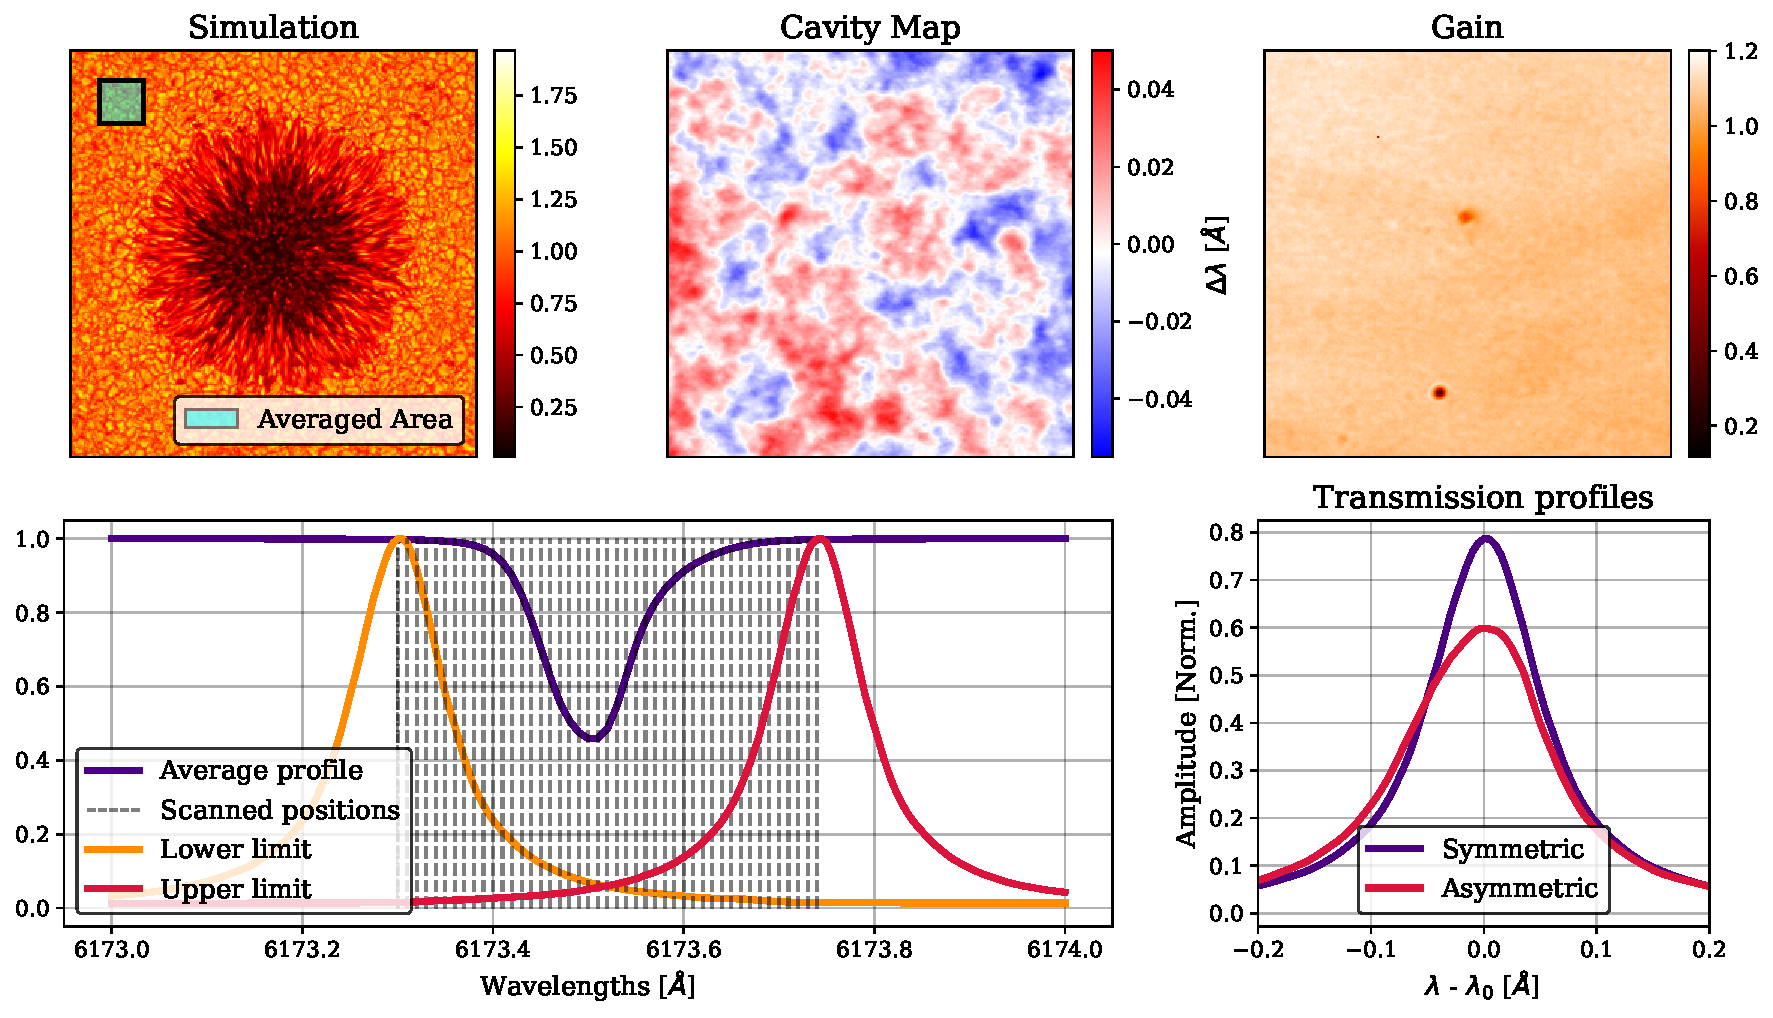
\includegraphics[width=\textwidth]{figures/Mancha/Inputs_mancha.pdf}
    \caption{
      Inputs for the simulation of the sunspot observation. The top row shows, from left to right, the continuum of the MHD simulation, the cavity map expressed as the corresponding shift in \r{A} and the gain map. The bottom row shows, again from left to right, a representation of the quiet-sun average profile with all the scanned wavelengths, and the transmission profile of the two different FPI configurations, the symmetric (perfect telecentric) and asymmetric (imperfect telecentric). The parametets employed for the etalon are: $R=0.892$, $n = 2.3268$, $d = 281$ $\mu m$, $f = 60$, $\Theta = 0^{\circ}$ (symmetric), $\Theta = 0.5^{\circ}$ (asymmetric).
      \label{fig_mancha: Inputs}}
\end{figure}

Although, in practice, it is not often possible to fully characterize the pre-filter, we assumed it has a rectangular shape centered at the wavelength of the observed spectral line ($\lambda _ {0}$) and a width of $2\Delta \lambda$ such that only one order of the etalon passes through. With this consideration, equation \eqref{eq_eta_corr: intensity} can be written as follows:

\begin{equation}
  I\left(\xi, \eta ; \lambda_{s}\right)=g(\xi, \eta)\int_{\lambda _ 0 - \Delta \lambda}^{\lambda _ 0 - \Delta \lambda} \iint  O\left(\xi_0, \eta_0 ; \lambda\right)  \mathcal{S}\left(\xi_0, \eta_0; \xi , \eta; \lambda-\lambda_{s}\right)  \mathrm{d} \xi_{0} \mathrm{~d} \eta_{0}\mathrm{d} \lambda \ .
  \label{eq_mancha: Intensity}
\end{equation}

For every tuned wavelength, the instensity in a given pixel is given by equation \eqref{eq_mancha: Intensity}, where the observed object is the sunspot simulation or the generated \textit{ideal} flat-field. 

The imaging response of the FPI is computed by solving the integrals in equation \eqref{eq_etalon_theory: electric_image_plane}. Given that we will account for the PSF in these simulations, numerical methods are necessary to evaluate the integrals. The computational burden is significant, as the integrals must be evaluated $N_{pixel} ^2 N_{\lambda} N_{mods} N_{sets} N_{cavities} > 2\times10 ^8$ times\footnote{$N_{pixels} = 561$, $N_{\lambda} = 45$, $N_{mods} = 2$, $N_{sets} = 2$, $N_{cavities} = 2$} for both sunspot and flat field observations. This extensive computation results in excessively long simulation times. To address this issue, a neural network was developed to reduce the computational time from \textcolor{red}{X to X}. The neural network was trained with known solutions to the integrals for a fixed set of etalon parameters, ensuring that its outputs are accurate to within 0.01\% for parameters within the training set.

In real-world scenarios, variations in pixel sensitivities (gain), in addition to the etalon imperfections (cavity map) are unavoidable. Including the effect of the gain into the simulation is straigghtforward as it only acts as a multiplicative factor that modifies the final intensity. In contrast, the effects of the cavity map are more cumbersome. Pixel-to-pixel variations in etalon defects shift the transmission profile of the FPI and must be accounted for when computing the imaging response. Both the gain and cavity map introduced in the simulations have been selected to resemble the real-case scenario of the SO/PHI instrument. The gain map (Fig. ~\ref{fig_mancha: Inputs} top right panel) utilized in the simulations is derived from a flat field of the SO/PHI-HRT instrument, and the cavity map employed (Fig. ~\ref{fig_mancha: Inputs} top central panel) is sourced from the cavity map of PHI's etalon.


\subsection{\label{sect: mancha_ff_corr}Flat-field correction.}

In principle, the flat-field correction is straightforward: first, the measured flat fields are normalized to preserve the spectral line information; and second, the observations for all tuned wavelengths are divided by the corresponding normalized flat field. However, in telecentric setups, this process is more challenging because flat-field observations are influenced by cavity errors, which can introduce additional artifacts into the measurements rather than (or in addition to) correcting them.


\begin{figure}
  \begin{minipage}[c]{0.7\textwidth}
    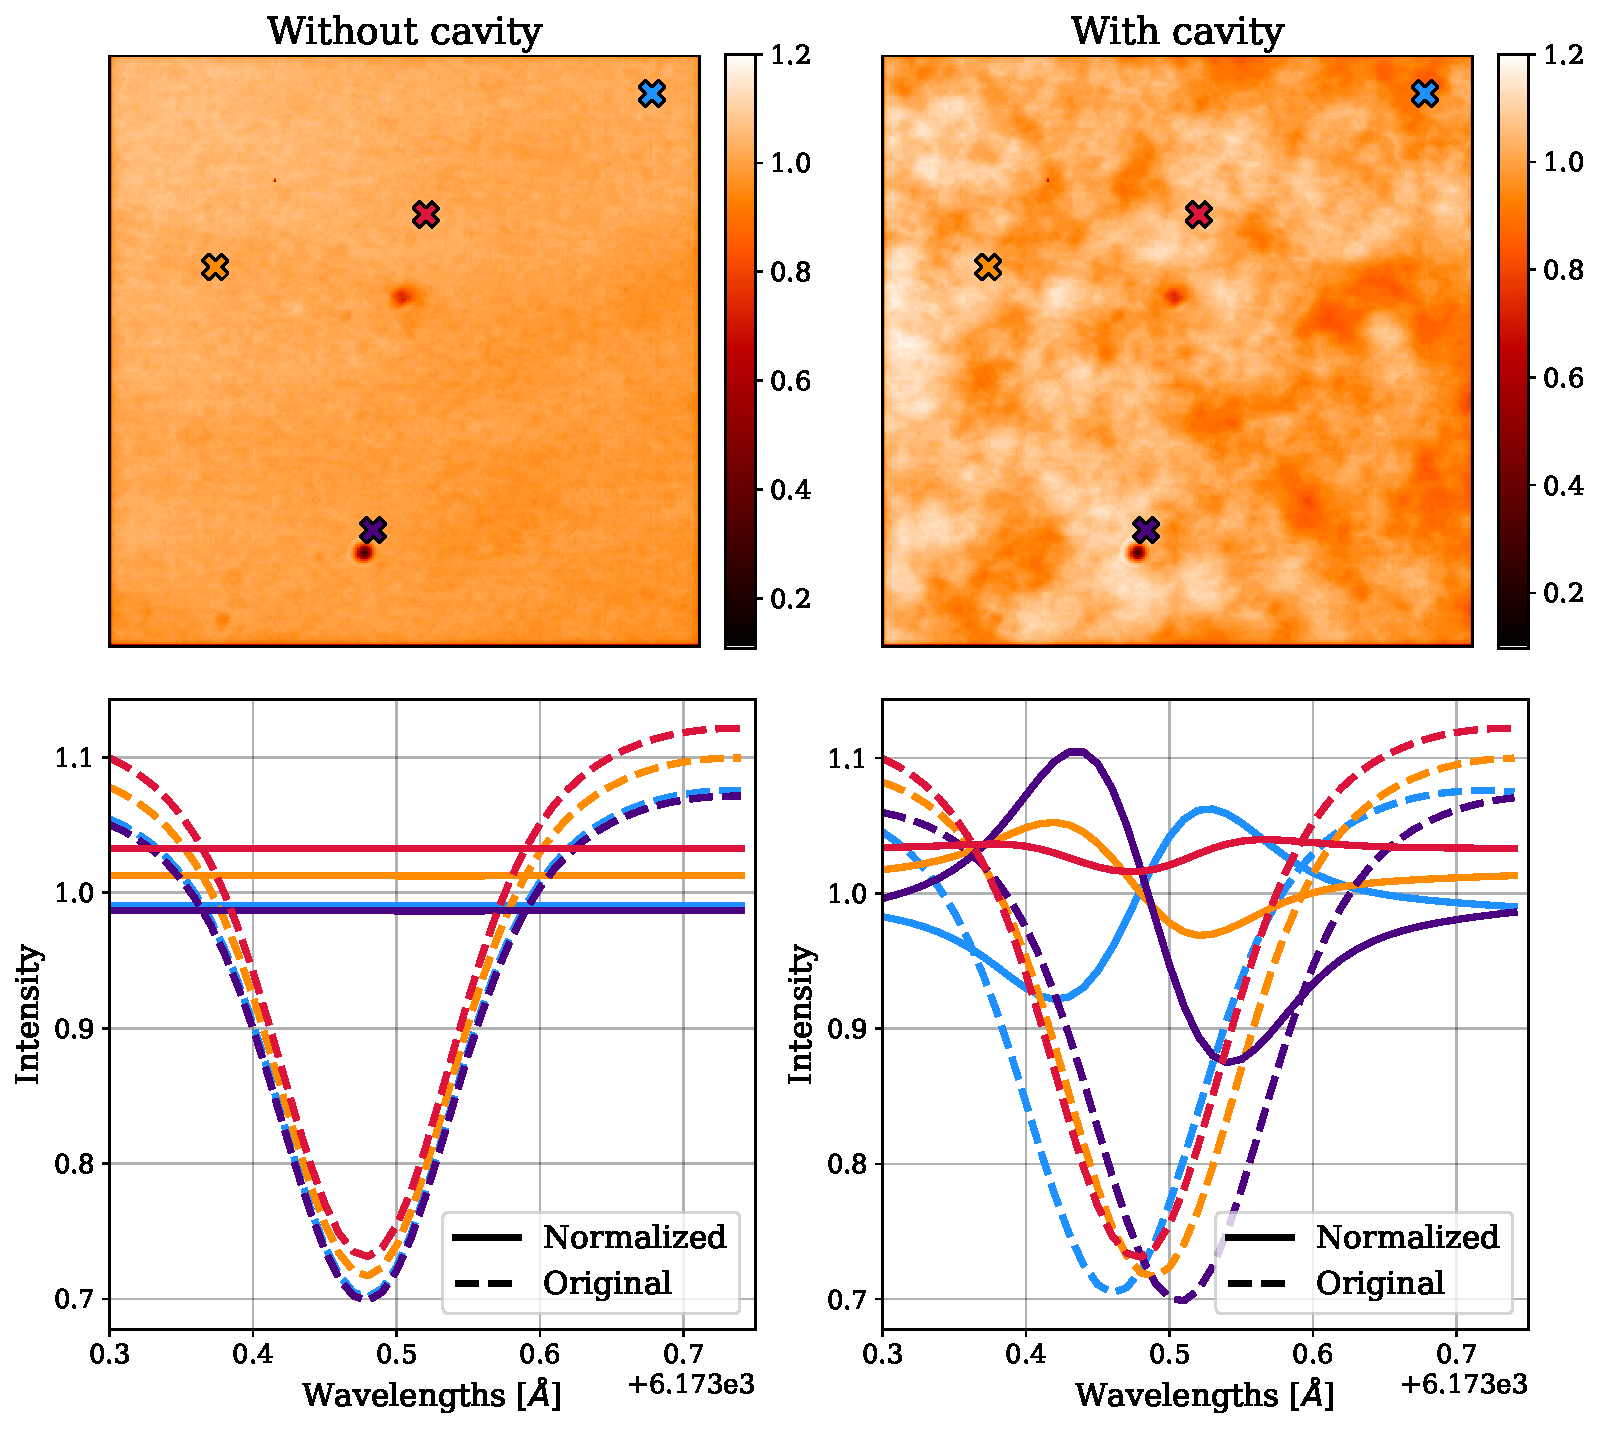
\includegraphics[width=\textwidth]{figures/Mancha/Flat_field_normalization.pdf}
  \end{minipage}\hfill
  \begin{minipage}[c]{0.27\textwidth}
    \caption{
      The top row shows the observed flat-fields at the core of the line for both the simulations without (left) and with (right) cavity. The bottom row shows the spectral profile of the pixels marked with an "X" of the corresponding color, for both scenarios, and before and after the normalization.      
    \label{fig_mancha: flat_field normalization}} 
  \end{minipage}
\end{figure}

Figure \ref{fig_mancha: flat_field normalization} shows the flat-fields observed at the core of the line for the simulations with and wihout cavity and the spectral profiles for a series of pixels. The effect of the cavity map in the flat-field observations is clearly displayed in both representations. In the flat-field itself, higher values of the cavity map appear brighter, as any displacement from the line core to either the blue or the red will result in an increase of the final intensity. In the spectral profiles, the pixels corresponding to higher values of the cavity error show a noticeably shift with respect to the rest position of the line core.   

From the normalized profiles, it is also evident that the normalized flats with cavity error will modify the profile of the observations once the division is carried out. Nevertheless, in order to correct for the effects of the cavity, the flat-field's spectral profiles cannot be flat as in the case without cavity, since we need to change the spectral information of the observations (shift the measured profile to the "correct" position). The problem arises when these flat-field not only shift the observed profiles but also (and very noticeably) modify their shape. 

\begin{figure}
  \begin{minipage}[c]{0.7\textwidth}
    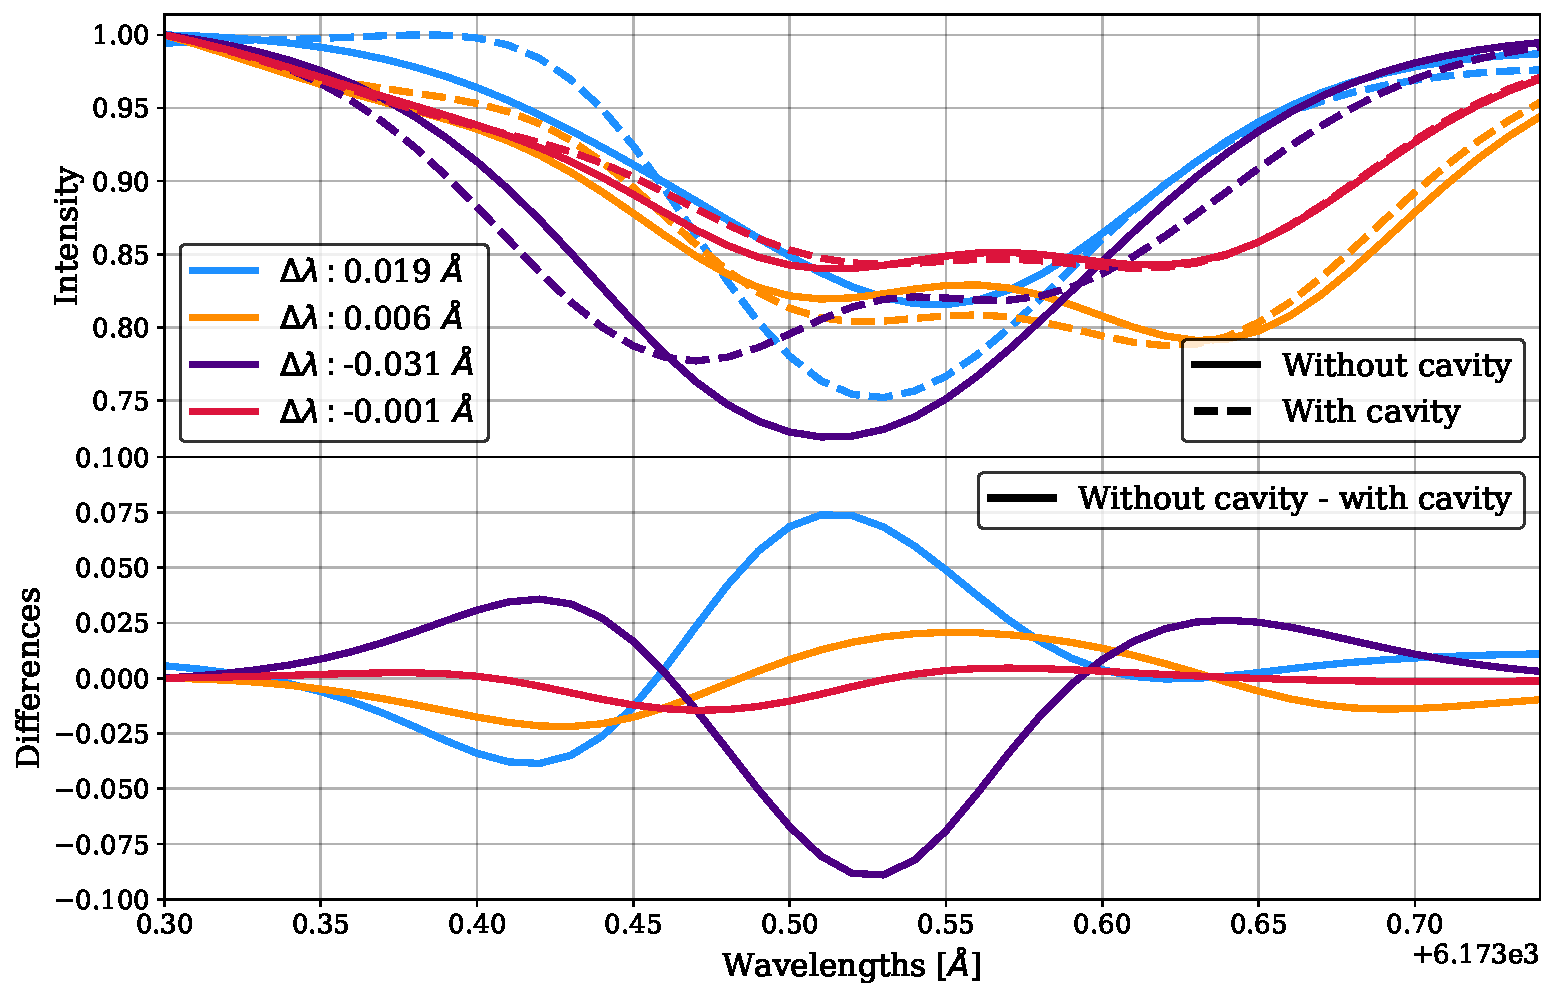
\includegraphics[width=\textwidth]{figures/Mancha/flatfield_norm_differences.pdf}
  \end{minipage}\hfill\hfill
  \begin{minipage}[c]{0.27\textwidth}
    \caption{
          The top panel shows four spectral profiles after the flat-field correction for the two scenarios, with and without cavity, and for the symmetric FPI. The selected pixels are the same than in Fig. ~\ref{fig_mancha: flat_field normalization}, and correspond to different values of the cavity map. The bottom panel shows the difference between the profiles with and witout cavities.
    \label{fig_mancha: Profiles_differences}} 
  \end{minipage}
\end{figure}

This problem is illustrated in Fig.~\ref{fig_mancha: Profiles_differences}, which displays the profiles after flat-field correction for both simulations, with and without the cavity map. Ideally, if the flat-field correction effectively compensates for the cavity errors of the FPI, the profiles from both scenarios should be identical or at least very similar. However, upon comparison, notable differences emerge, particularly for pixels with high cavity map values (light blue and dark blue lines). These profiles are not only shifted but also exhibit changes in shape. 

This challenge is why some data reduction pipelines adopt a different approach. Instead of using the flat-fields of the corresponding wavelengths, only the continuum flat-field is employed for the correction. When the continuum is measured sufficiently far from the spectral line, it remains unaffected by any spectral shift. By using this measurement, one can correct for spurious effects unrelated to spectral shifts, such as pixel sensitivity variations or dust grains. However, this method does not correct for the effects of the cavity.

If the cavity map is thought to be known, the velocity associated with the spectral shift caused by the cavity can be calculated. This "velocity-error" map can then be used to correct the Doppler velocity map derived from the observations that have not been corrected for the cavity map. Theoretically, this approach should address the cavity effects in velocity calculations. Nonetheless, potential impacts of the cavity map on magnetic field calculations remain uncorrected, as the relationship between wavelength shifts and magnetic fields is not as straightforward as in the case of velocity.

\subsection{\label{sect: mancha_vlos}Velocity maps}

We begin our analysis by studying the LOS velocities and the errors associated with their computation. These velocities are derived from the spectral shift of each profile relative to the rest position of the spectral line, using the Doppler formula (Eq.~\eqref{eq_spectro: Doppler}). Given that this computation relies exclusively on the spectral shift, it is particularly susceptible to errors caused by cavity effects.

According to the center-of-gravity method \citep{center_of_gravity}, the central wavelength of a given spectral profile, $\lambda _ {COG}$, can be computed from:

\begin{equation}
  \lambda _ {COG} = \frac{\int \lambda \left( I _{cont} - I\right)d\lambda}{\int \left( I _{cont} - I\right)d\lambda}. 
\end{equation}

Once $\lambda _ {COG}$ has been determined, the spectral shift of the corresponding profile will be given by $\Delta \lambda = \lambda _ 0 - \lambda _ {COG}$. 

We have computed the velocities employing the two flat-field correction strategies mentioned in the previos section: the "standard" approach, where each observation is corrected with the flat-field of the corresponding wavelength; and the "continuum" approach, where only the continuum flat-field is employed. Figure \ref{fig_mancha: int_and_vlos_examples} shows the continuum intensity and the velocity maps obtained for both strategies in the top row.  

\begin{figure}
  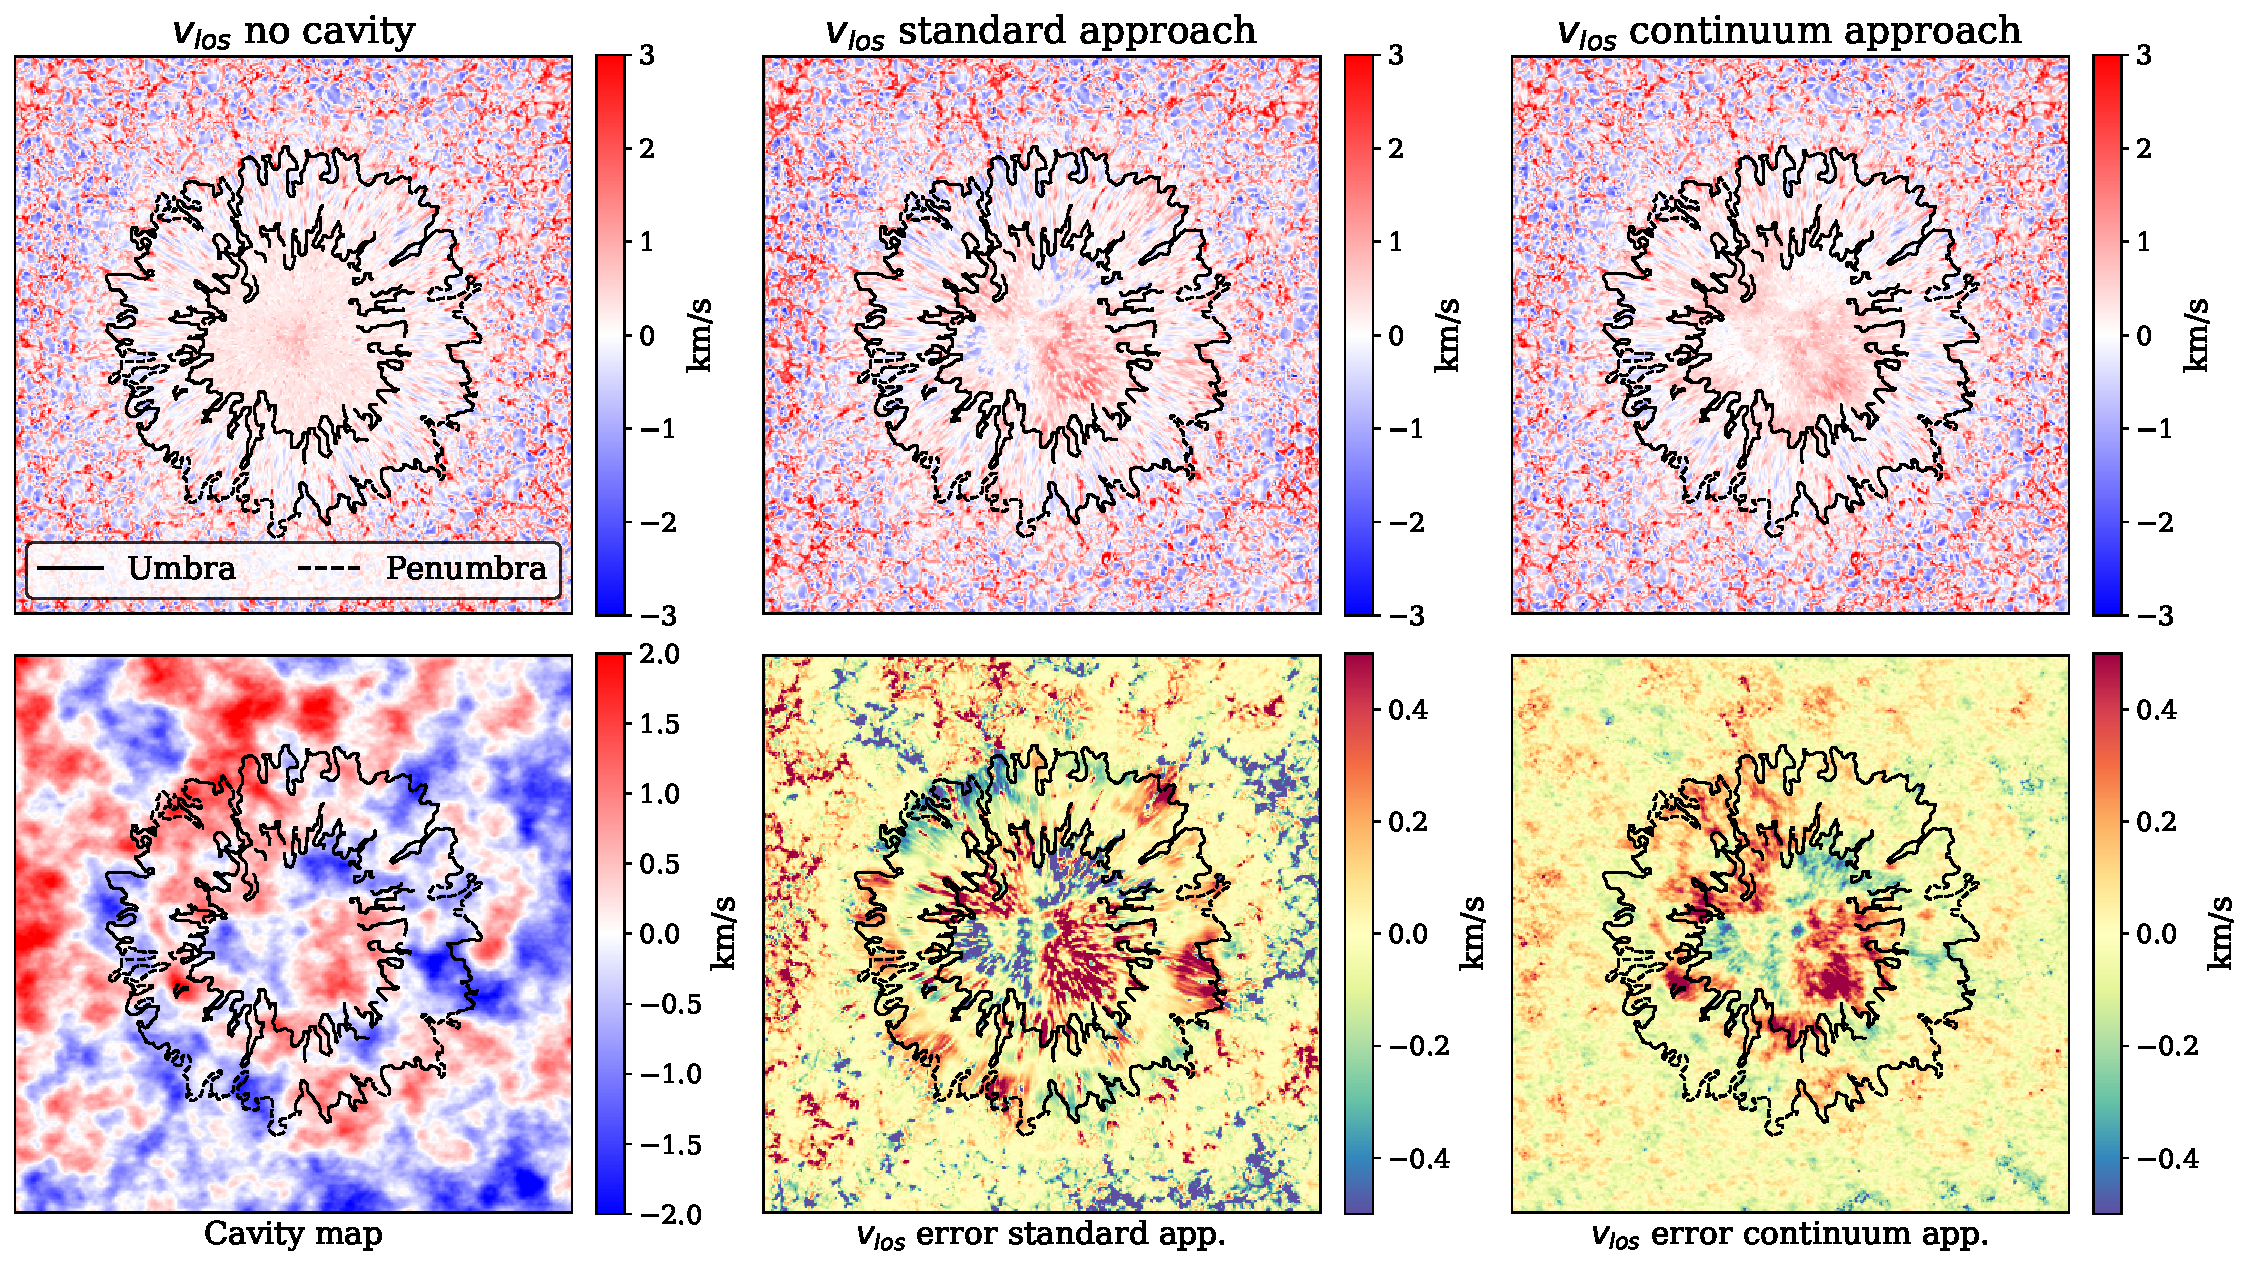
\includegraphics[width=\textwidth]{figures/Mancha/intensity_and_vlos_examples.pdf}
  \caption{
    The top row shows, from left to right, the observed intensity in the continuum, the LOS velocity for for the standard approach and the LOS velocity for the continuum aproach, all three for the symmetric FPI and belonging to the simulations with cavity map. The bottom row shows, again from left to right, the velocity error associated with the cavity map, the error for the LOS velocity for the standard approach and the error for the LOS velocity of the continuum approach. The error is computed by substracting the measrument to the reference. All representations show the boundaries of the umbra and penumbra for an easier identification of the regions in the velocity and cavity maps.   
    \label{fig_mancha: int_and_vlos_examples}}
\end{figure}

At first glance, the velocities derived for each approach might look identical, but under closer inspection, some differences arise. In order to highlight these differences and to asses the accuaracy of the obtained velocities we will compare them to the velocity obtained in the scenario where no cavity map was introduced. Figure \ref{fig_mancha: int_and_vlos_examples} shows this comparisons in the bottom row, along with the cavity map with the umbra and penumbra overplotted to be able to align the error with the cavity.   

The error in the velocity computation shows that the effects of the cavity map remain uncorrected in the observations. Both correction approaches exhibit errors with structures corresponding to the cavity map. For the standard correction, this effect is pervasive throughout the field of view (FoV), whereas for the continuum approach, it is primarily concentrated in the umbra, although other regions also exhibit this behavior.

Moreover, the errors are notable, given that regions of the penumbra show errors of around 10\%. Errors in the umbra are similarly significant in percentage terms; however, studies of these regions are less frequent due to their low SNR resulting from their inherent darkness. Conversely, extensive research exists on the flows observed in the penumbra (\textcolor{red}{Ref XX??}), prompting us to prioritize investigation in this area.

\begin{figure}
  \begin{minipage}[c]{0.7\textwidth}
    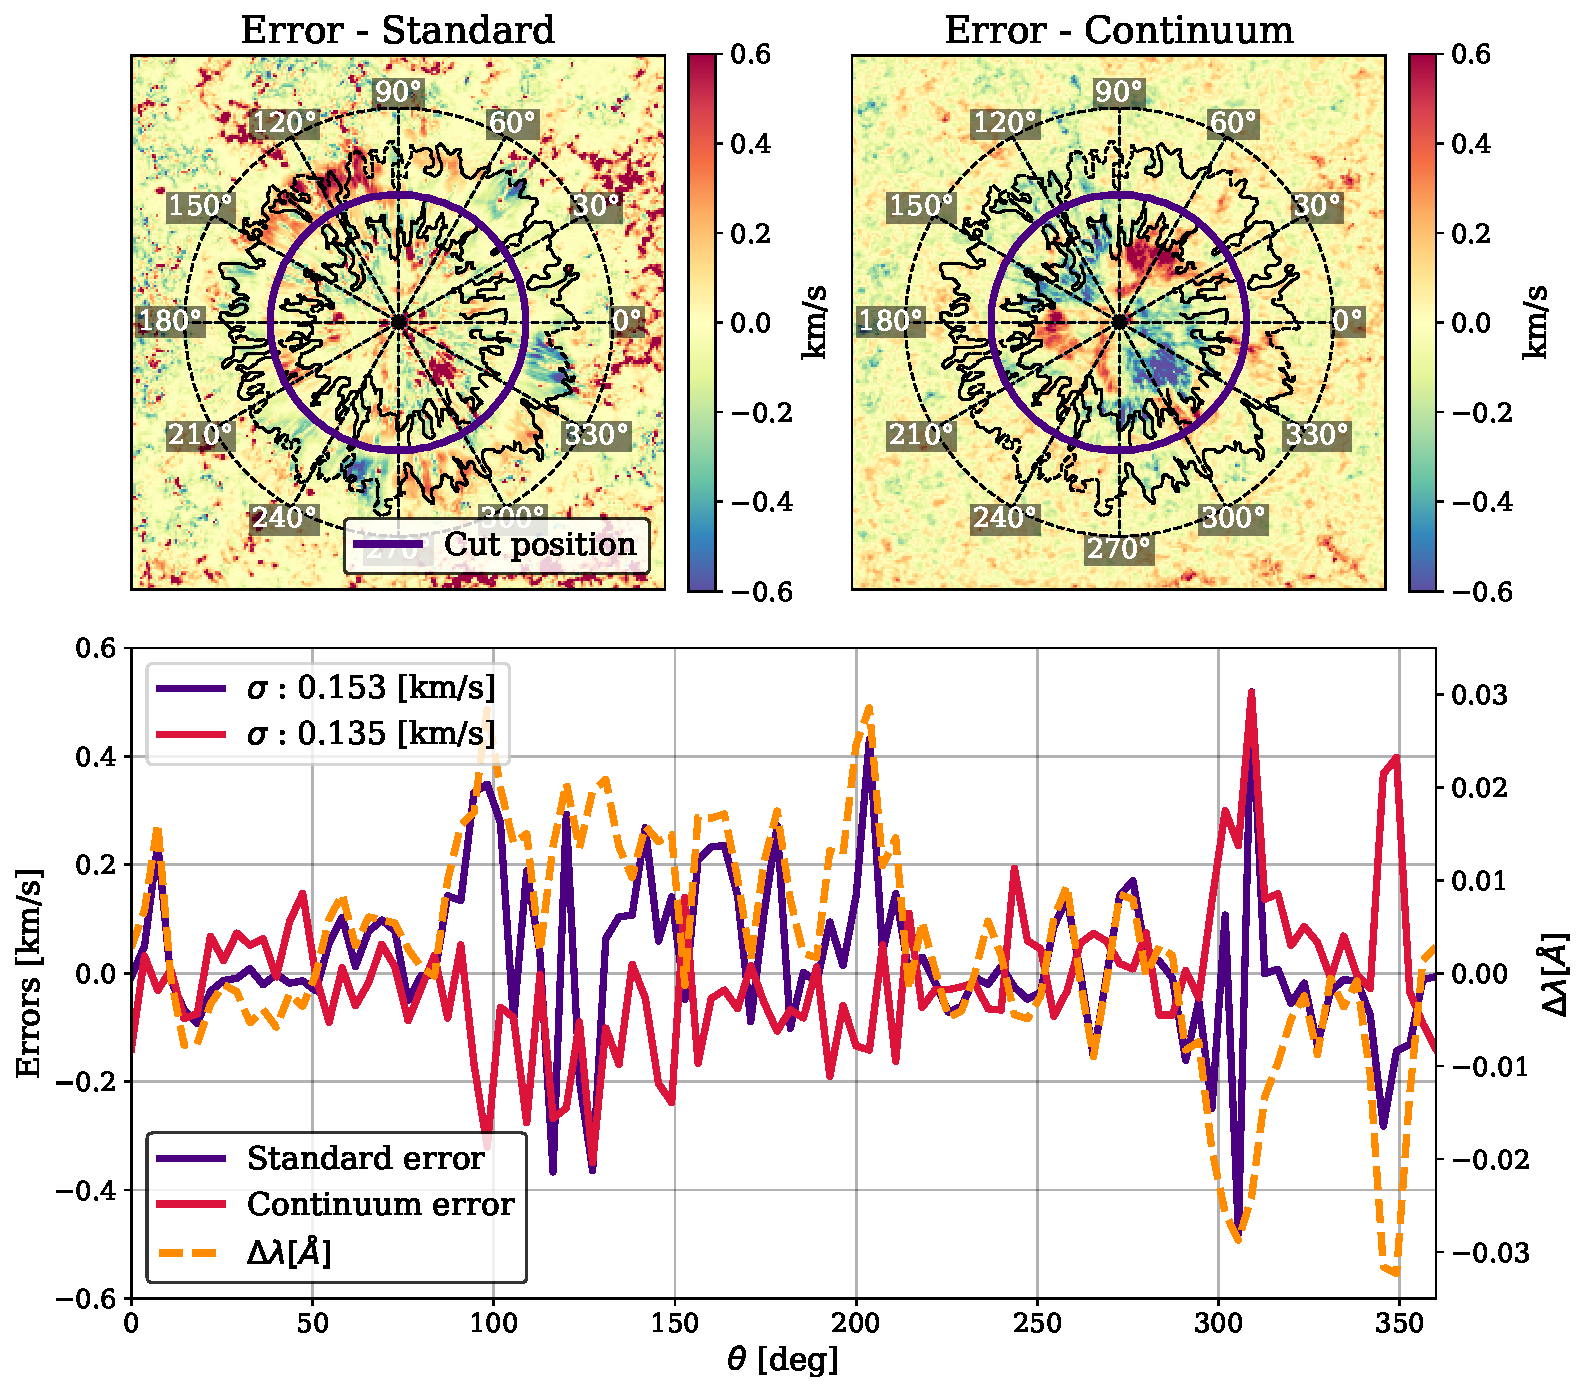
\includegraphics[width=\textwidth]{figures/Mancha/circular_cut_standard_cont.pdf}
  \end{minipage}\hfill\hfill
  \begin{minipage}[c]{0.27\textwidth}
    \caption{
      The top row shows the velocity error maps for both the standard and continuum approaches, along with the cut position and an overlay of the degrees for easier interpretation of the plotted profiles. The bottom panel shows the velocities along the cut for both aproaches along with the value of the cavity map at the corresponding position.\label{fig_mancha: verror_circular_cut}} 
  \end{minipage}
\end{figure}

A more quantitative analysis is shown in Fig. \ref{fig_mancha: verror_circular_cut}, where the velocity error along a circular path is shown, for both approaches, in addition to the associated spectral shift of the cavity values at identical positions. This representation clearly demonstrates the correlation between the structural features of the cavity map and the velocity error. For both approaches, with a more pronounced effect observed in the standard approach, the absolute value of the error escalates with increasing spectral shifts of the cavity.

\textcolor{red}{It is evident from the previous analyses that the approach of flat-field correction affects the resulst as differences are observed between correction approaches, but what about the FPI's transmission profile? It is common practice to neglect the assymetric nature of real telecentric mounts in most data reduction pipelines beacuse the possible effects of the assymetries of the profiles are assumed to be negligible.} 

\begin{figure}
  \begin{minipage}[c]{0.5\textwidth}
    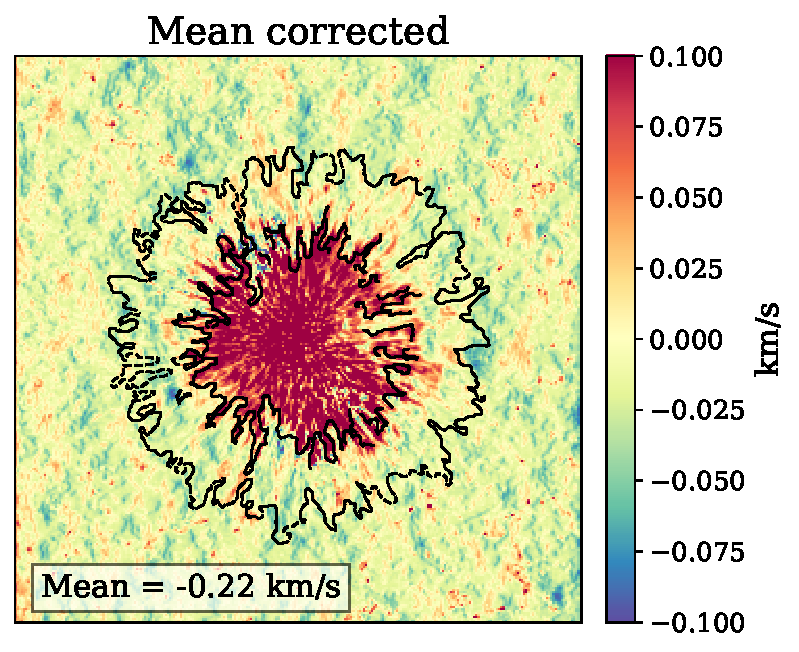
\includegraphics[width=\textwidth]{figures/Mancha/vlos_sym_vs_asym.pdf}
  \end{minipage}\hfill\hfill
  \begin{minipage}[c]{0.47\textwidth}
    \caption{
      Difference in LOS velocities between the symmetric and assymetric FPIs (symmetric - asymmetric). The mean value of the difference has been substracted for the whole FoV. \label{fig_mancha: vlos_asym_vs_sym}} 
  \end{minipage}
\end{figure}

Figure X depicts the differences in the computed velocities for the symmetric and assymetric FPIs. The main effect of the assymetry is a systematic shift of the profile measurements towards the red wing of the spectral profile, due to its higher transmissivity than its blue counterpart. This shift results in an average difference of around $0.2$ km s$^{-1}$ that can be seen over the whole FoV. 

This systematic shift can be removed from the velocities computed with the assymetric FPI by substracting the average difference between symmetric and assymetric velocities. The panel XX of figure XX, shows the difference following this correction has been carried out. Despite accounting for the systematic shift, discrepancies are still present, predominantly within the umbra, though they are observed across the entire FoV. The umbra is again more sensible than other regions, displaying the highest error in the whole map, mainly exhibiting a shift towards the \textcolor{red}{BLUE?}, for the assymetric scenario. Outside the umbra, differences are smaller, reaching up to 100 ms$^{-1}$, typically trending towards the red.

The fact that the umbra exhibits different behaviors compared to the rest of the FoV, along with the difference nted between the two types of FPIs, suggests that the amplitude and behavior of these effects are sensitive to the shape of the spectral profile and the FPI's transmission profile. 

\subsection{\label{sect: mancha_blos}Magnetic field maps.}

It is expected that cavity errors significantly impact velocity calculations, as these are derived solely from the analysis of spectral shifts. However, the effect of these errors on the calculation of the magnetic field is not as straightforward as its determination involves not only the spectroscopy, but also polarization. 

To calculate $B_{LOS}$, we need to determine the circularly polarized component of the light. This requires demodulating the simulated observation using a process analogous to that described in the TuMag pipeline (ref XXX). Once the stokes components have been determined, the LOS strength of the magnetic field is computed using the center-of-gravity method  (eq.~\eqref{eq_spectro: Blos-cog}). 

\begin{figure}
  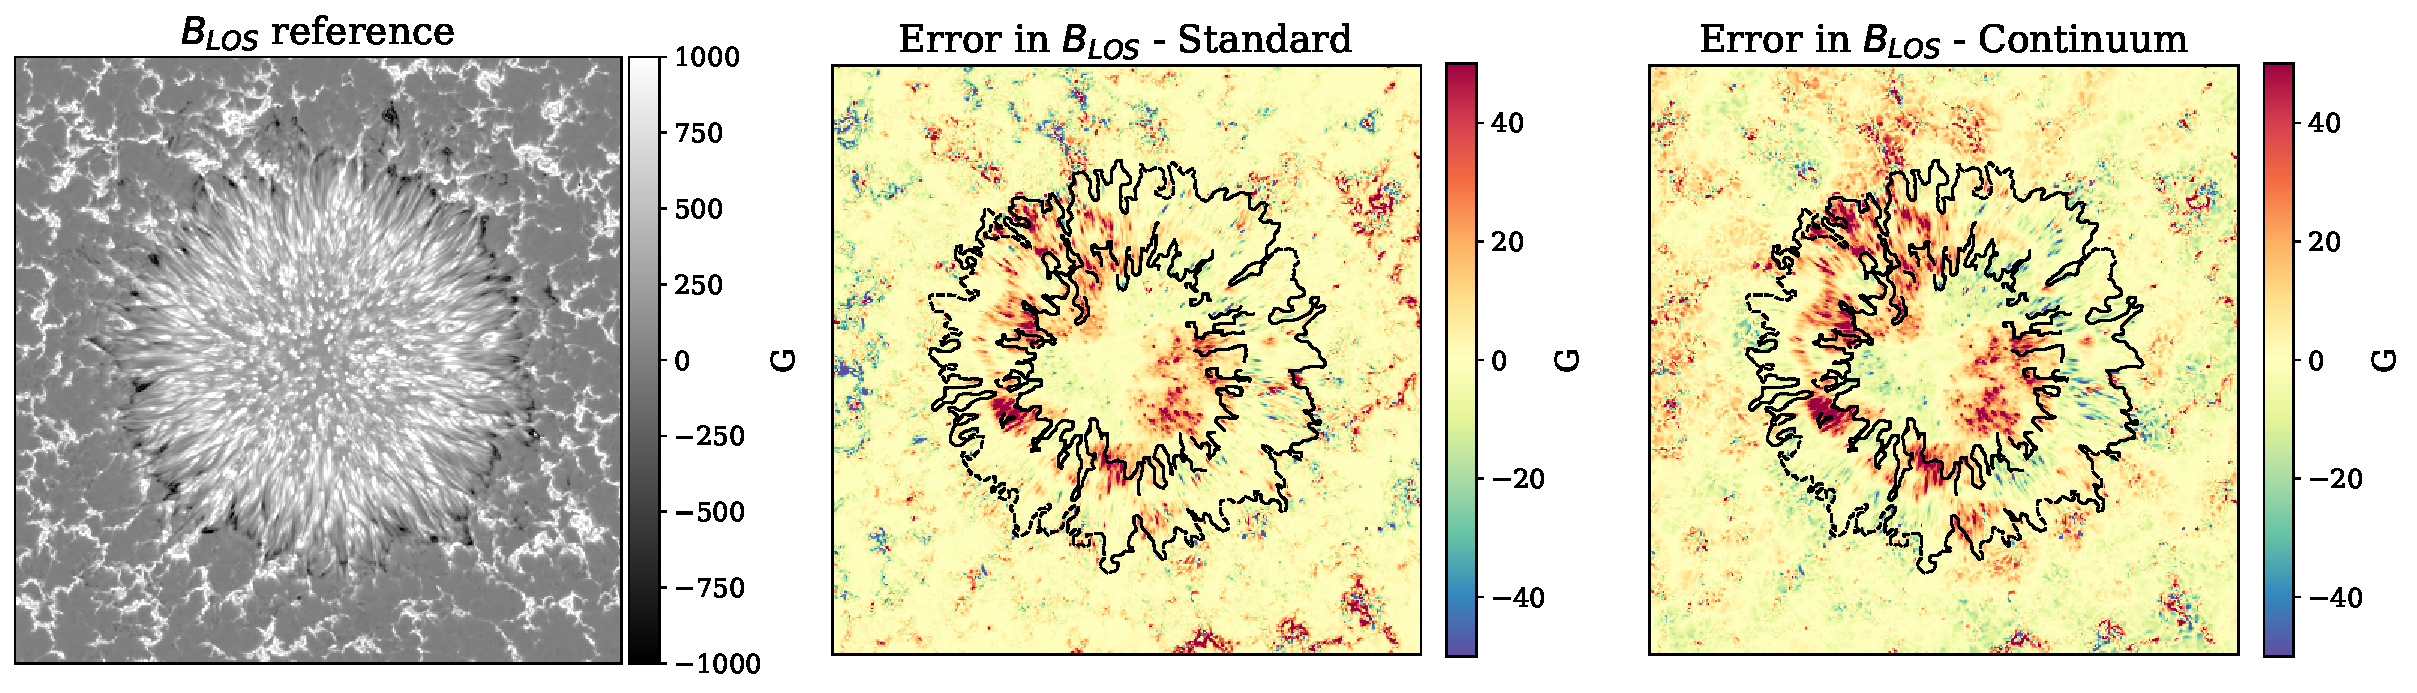
\includegraphics[width=\textwidth]{figures/Mancha/blos_errors.pdf}
  \caption{
    From left to right, $B_{LOS}$ for the simulation with no cavity and a symmetric FPI, error in $B_{LOS}$ computation for the standard approach with a symmetric FPI, and error in $B_{LOS}$ computation for the continuum approach with a symmetric FPI. 
    \label{fig_mancha: blos_errors}}
\end{figure}

Figure \ref{fig_mancha: blos_errors} shows the LOS strength of the magentic field for the simulation with no cavity (the one employed as reference) and the errors in its calculation for both flat-fielding approaches.  In the continuum approach, the structures observed in the error map closely resemble those in the cavity map. This similarity is expected since no correction has been applied to account for the cavity error. While it is possible to compute the velocities associated with the spectral shift caused by the cavity map, this is not feasible for the magnetic field. Consequently, any effect of the cavity remains in the data when using the continuum approach.

As a result, errors in the magnetic field computation appear larger or more prevalent across the entire field of view (FoV) for the continuum approach. Although small, these residuals of the cavity map in the magnetic field map are one of the main problems of employing the continuum apprach in real data. 

However, for both correction strategies, the errors remain relatively small, reaching values of approximately 3 G, compared to magnetic field signals of around $\pm 100$ G. 

\section{\label{sect: etalon_corr_fitting}Fitting algorithm}

Results from the previous section highlight the relevance of carefully addressing the data correction of FPI-based instruments. Although some pipelines address these deviations by correcting them only at first order through a regular flat-fielding procedure with no further computations, the residues left in the data can lead to errors as high as those shown in the previous section, depending on the FPI's properties. For this reason, different approaches have been taken to address these additional corrections. Typically, each instrument has a specific data reduction pipeline where the corrections are carried out taking into account the individual properties of the instruments, hence giving rise to different methods. An example of a more detailed calibration pipeline can be found in \cite{crisp-method}. By using a simplified analytical expression for the etalon transmission profile, Schnerr et al. were able to extract from the flat fields the contributions caused by the FPI cavity errors and variations in reflectivity for the CRISP instrument, which are then taken into account in the data calibration.

For the first order, this is a good approximation, but since asymmetries in the transmission profiles naturally arise in telecentric instruments \citep{franI}, deviations originating from them cannot be fully corrected. Thus, knowledge of the exact shape of the transmission profile is necessary to fully account for these deviations. \cite{schamer_method} already allowed asymmetries to be dealt with in the pipeline of the CRISP instrument, but the asymmetries originated from wavelength shifts induced by two distinct etalons, or from an angular dependence along the FoV introduced to approximate the behavior in telecentric setups.  

We aim to further extend and generalize the strategy employed in \cite{crisp-method} and \cite{schamer_method} by including the exact shape of the transmission profile for the telecentric configuration in the analysis. By doing so, we can fit and take into account the presence of asymmetries in the profile that arise in these setups due to an asymmetric pupil apodization. We have developed a method for deriving the etalon properties from the data in such a way that prior knowledge of the distribution and magnitude of the defects is not needed. We do not make any distinction between defects associated with the mirror's flatness or separation, refraction index, or cavities. This way, we ensure the applicability of the algorithm to all types of FPIs (air and solid). Our technique also differentiates the effects associated with the etalon from other corrections not related to it, such as pixel-to-pixel variations of the gain across the detector. By comparing the theoretical prediction, obtained through the analytical expressions of the transmission profile, with the measured data, we can disentangle the etalon properties from the flat-field observations. 

In this section, we introduce the algorithm and evaluate its performance. We begin by outlining the approximations made and detailing the algorithm in Sections \ref{eta_corr_susec: approx and simulations} and \ref{eta_corr_susec: fitting algorithm}, respectively. The method was tested on a series of simulated observations with controlled configurations to evaluate the impact of different observational properties on the accuracy of the results. Finally, the algorithm was applied to a dataset from the HRT telescope of the SO/PHI instrument to assess its performance in real scenarios. The results for both the simulated scenarios and real data are discussed in Section \ref{eta_corr_susec: results}.

\subsection{\label{eta_corr_susec: approx and simulations}Initial approximations and observations simulation.}

As initial approximations, we will adopt the same assumption regarding the prefilter as used in the sunspot simulation; specifically, that it has a rectangular shape with a width such that only one order of the etalon is let through. Additionally, we will disregard the spatial PSF of the FPI and assume that the spatial dependence can be represented by a Dirac delta function to simplify the equations. Therefore, if we assume that the image response of the FPI follows the expression:
\begin{equation}
S\left(\xi_0, \eta_0; \xi , \eta; \lambda-\lambda_{s}\right)=\delta(\xi_0-\xi,\eta_0-\eta)\Psi(\xi,\eta,\lambda-\lambda_s),
\end{equation}
equation \eqref{eq_mancha: Intensity} simplifies into:
\begin{equation}
    I\left(\xi, \eta ; \lambda_{s}\right)=g(\xi, \eta)\int_{\lambda _ 0 - \Delta \lambda}^{\lambda _ 0 + \Delta \lambda} O\left(\xi, \eta ; \lambda\right) \Psi\left(\xi, \eta ; \lambda-\lambda_{s}\right)  \mathrm{d} \lambda.
    \label{eq_eta_corr: intensity}
\end{equation}

The explicit shape of $\Psi$ varies depending on the optical configuration of the instrument, whether collimated or telecentric. Specifically, we will employ three types of transmission profiles: one for the collimated configuration, one for a perfect telecentric setup (normal incidence), and one for an imperfect telecentric setup. The first two have analytical expressions for the transmission profile in the absence of the spatial PSF, as detailed in Sections \ref{susec_etalon_theory: collimated} and \ref{susec_etalon_theory: Tele-perfe}, respectively. For the imperfect telecentric configuration, the transmission profile must be determined numerically (see Section \ref{etalon_theory: Tele-imperfe}).
  
We have tested the perforamnce of the algorithm on a series of simulations of a spectral line observation in different conditions. We used the Kitt Peak FTS-Spectral-Atlas as the reference \citep{fts} and, specifically, the Fe I spectral line at 6173.3~\r{A}. Each observation was composed of $N_\lambda$ wavelengths, where the measured intensity was recorded. At every wavelength $\lambda_s$, the corresponding transmission profile of the etalon $\Psi^{\lambda_s}$ was computed, and the "observed" intensity $I ^{\lambda _ s} _ {{\rm obs}, i}$ corresponding to a specific spatial location $(\xi, \eta)$, represented hereinafter by the pixel $i$, was calculated using Eq.~\eqref{eq_eta_corr: intensity}. Additionally, we took into account the presence of additive Gaussian noise. This noise does not necessarily respond to any parameter fluctuation within our analytical expressions or photon noise but comes from any unexpected variations that may not have been modeled in the theoretical scheme.

Additionally, we included the presence of defects arising from irregularities or inhomogeneities on either the cavity thickness $d$, the refractive index $n$, or from deviations of the angle of incidence $\theta$. In order to simulate this, we introduced a relative perturbation $\Delta a$ into the etalon equation that accounts for any local deviation of the value of $a$ with respect to its nominal value. This parameter changes from pixel to pixel differently for the collimated and telecentric configurations. In the former, the profile shifts across the FoV only because of the different incidence angles of the light beam on the etalon. In the latter, local variations of $n$ and/or $d$ are mapped directly onto the detector. We also note that variations in the incidence angle must be considered as well when the degree of telecentrism varies along the detector. Analytically, the parameter $a$ at each $i$-th pixel is given by $a' _ i = a \Delta a _ i$, where $a = (2\pi/\lambda) n d\cos\theta$ is constant along the FoV. Note that rewriting the equations for the transmission profiles (sections \ref{susec_etalon_theory: collimated} and \ref{susec_etalon_theory: Tele-perfe}) using this definition of $a$ is straightforward. In collimated configurations, the parameter $\delta$ (eq. \eqref{eq_etalon_theory: collimated_delta}) is simply $2a$. In perfect telecentric configurations, $\theta$ is always 0, so the given transmission profile is already expressed in terms of $a$.   

We let $n _ i ^{\lambda_s}$ be the  noise contribution at the $i$-th pixel and wavelength $\lambda_s$. Thus, the observed intensity at that pixel when the etalon is tuned at $\lambda _s$, $I ^{\lambda _ s} _ {{\rm obs}, i}$ is given by 
\begin{equation}
I ^{\lambda _ s} _ {{\rm obs}, i} = g_i \frac{\int_{\lambda_0 - \Delta \lambda}^{\lambda_0 + \Delta \lambda} O(\lambda)\Psi^{\lambda _ s} (\lambda , \Delta a _i)  d\lambda}{\int_{\lambda_0 - \Delta \lambda}^{\lambda_0 + \Delta \lambda} O(\lambda)\Psi^{\lambda _ c} (\lambda, \Delta a _ i)  d\lambda} + n _ i ^{\lambda_s}    ,
\label{eq_eta_corr: Profile - General}
\end{equation}
with $\lambda _ c$ being the continuum wavelength. From a practical point of view, the integration limits are set in such a way that only a single resonance (or order) of the etalon is included with the limits, thus, acting akin to the sorting pre-filter commented on previously. We note that the denominator strictly corresponds to the intensity at the continuum of the line in the absence of the transmission profile or if the continuum wavelength is far enough from the spectral line. In any other case, the transmission should be taken into account as well to normalize the observations to the local continuum, which is necessary since we work with relative measurements. An example of a spectral line measurement is displayed in Fig.~\ref{fig_etalon_corr: Prof-Measure}.
\begin{figure}
    \centering
    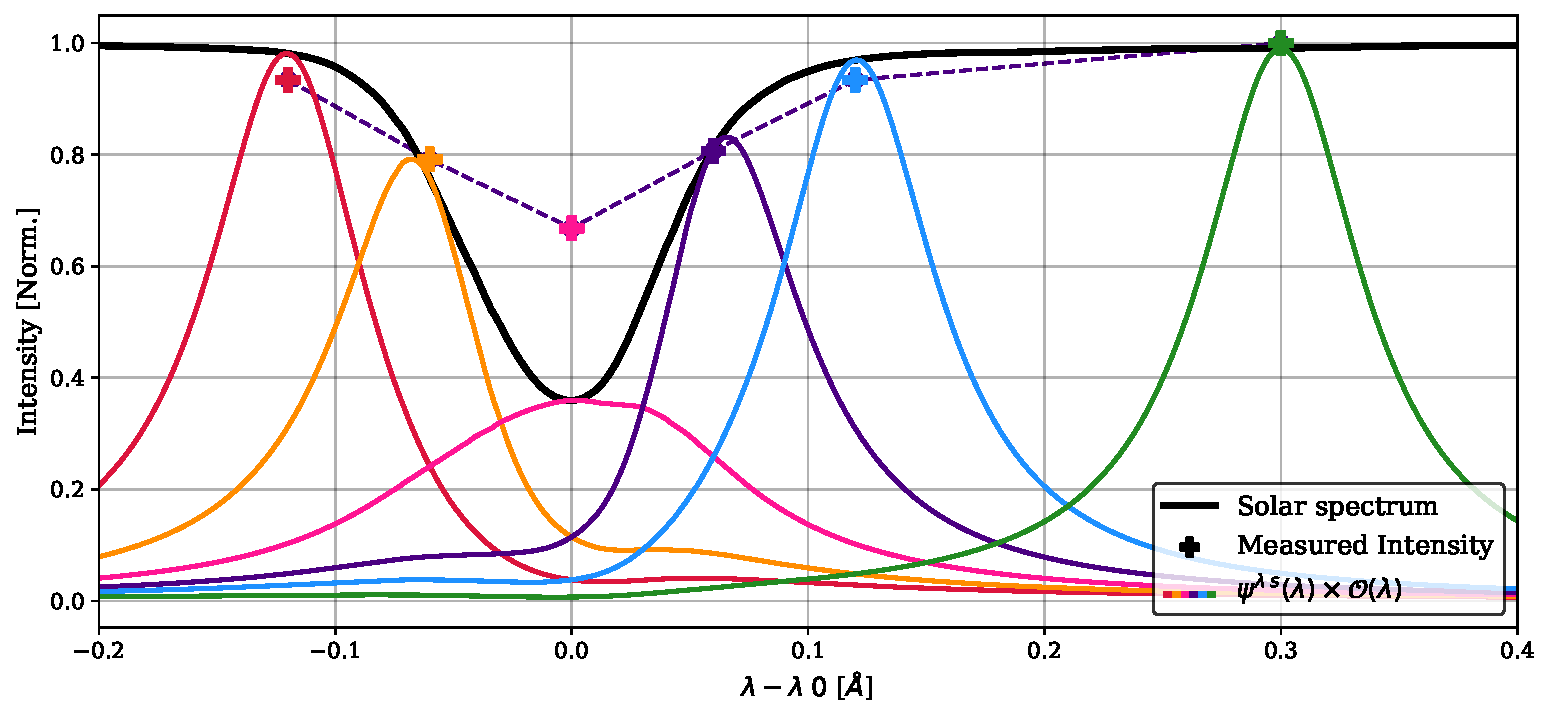
\includegraphics[width = \textwidth]{figures/EtalonPaper/ProfileMeasurement.pdf}
    \caption{Simulated observation of the Fe I spectral line ($\lambda _ 0 = 6173.3$\r{A}) using a collimated mount and a total of $N_ \lambda = 6$ wavelengths that have been equally distributed along the spectral line, with the exception of the continuum measurement (light blue), which is selected at $300$ m\r{A} from the blue of the line core. The measured intensity is the result of computing the value given by Eq.~\ref{eq_eta_corr: Profile - General} at each wavelength and with $g = 1$.
    } \label{fig_etalon_corr: Prof-Measure}
\end{figure}

For both the collimated and telecentric configurations, we modeled etalon and gain imperfections over a $100\times100$~px$^2$ image. Pixel-to-pixel variations in the sensor efficiency were modeled following a random spatial distribution, as shown in Fig.~ \ref{fig_etalon_corr: Inputs} (top panel). Additionally, we included a set of pixels with very low gain values, which represent a group of dead pixels or dust grains.

We modeled the etalon defects as changes in $\Delta a$ in such a way that the maximum displacement reaches $3$ pm. The spatial distribution of the values of  $\Delta a $ follows an increasing radial distribution, as shown in Fig.~ \ref{fig_etalon_corr: Inputs} (bottom panel). Such a spatial distribution coincides with the expected one in collimated etalons due to the change in the incidence angle across the FoV. Telecentric mounts do not exhibit a spatial distribution of their defects such as this, but using the same spatial distribution in the two cases allowed us to compare the performance of the method for both setups in a systematic way. Since $\Delta a$ accounts for relative perturbations, it is by definition an adimensional parameter. However, to grant it a physical meaning, we express the values of $\Delta a$ in \r{A}, representing the associated shift of the transmission profile with respect to the original position determined by $a$.

\begin{figure}
  \centering
    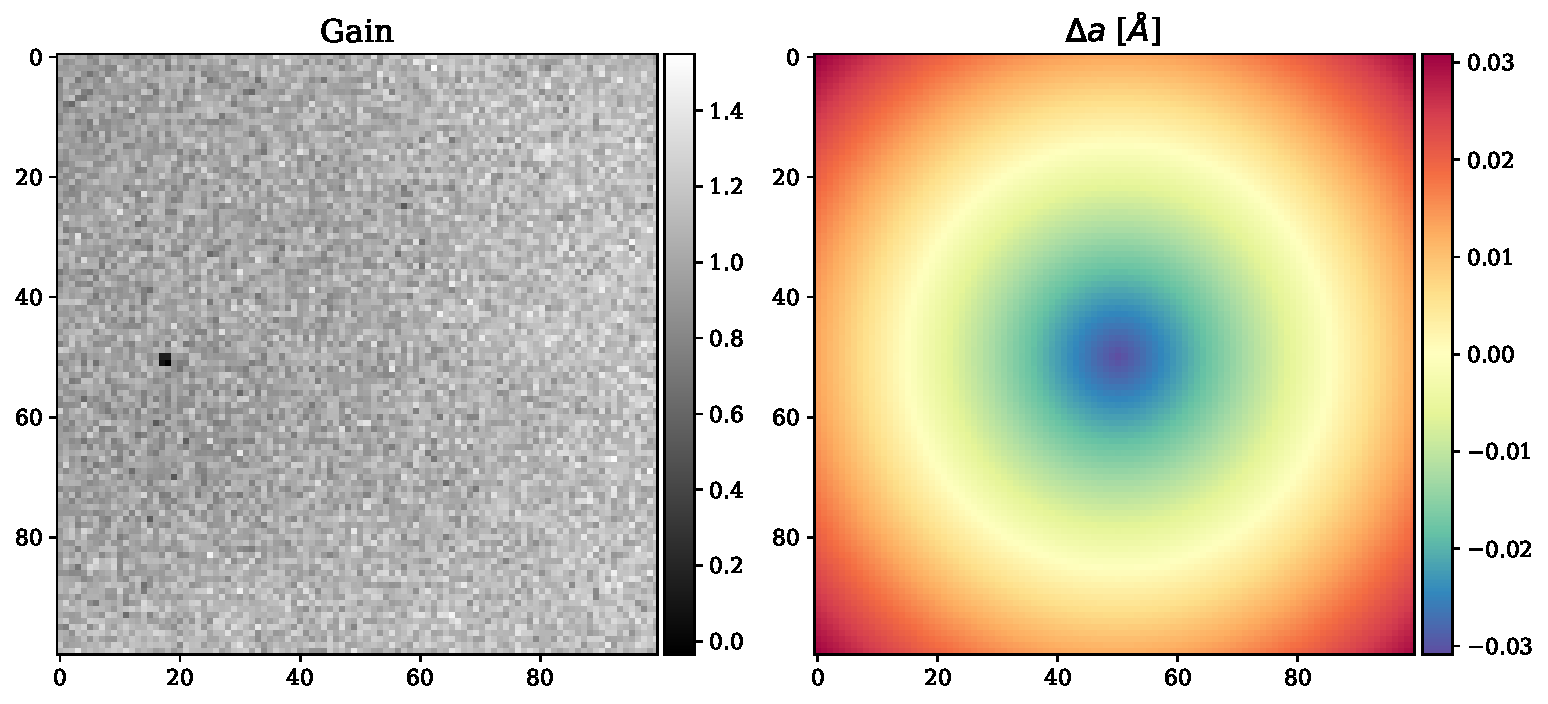
\includegraphics[width=\textwidth]{figures/EtalonPaper/Gain_Da_Inputs.pdf}
    \caption{
      Input maps introduced when simulating the observations. The left panel represents the gain generated as white Gaussian noise, with values ranging from 0.8 to 1.2. A dust speck was introduced by creating a group of four pixels with low values of $g=0.2$ for the gain. The right panel shows the spatial distribution of the defects in the etalon. The distribution follows a radial pattern starting from the center of the FoV. The defects vary from $0\,\%$ deviation to up to $5\times 10 ^{-4}\,\%$, which corresponds to a shift of 3~pm. Both possible directions for the deviations have been considered. The sign of the deviation is negative at the very center, which introduces a redshift, while it is positive at the corners, causing a shift of the profile into the blue.
      \label{fig_etalon_corr: Inputs}}
\end{figure}

\subsection{\label{eta_corr_susec: fitting algorithm}Fitting algorithm}

We have developed an algorithm able to extract the distribution of the etalon defects and the gain map from data taken by etalon-based instruments, which enables the correction of the two contributions separately. The algorithm works by minimizing a given merit function that depends on the gain and the etalon defects. 

In particular, we have defined an error metric, $\varepsilon  ^\lambda$, at each tuned wavelength, computed by comparing the measured intensity with the theoretical prediction. If we let $I_ {i, {\rm obs}} ^{\lambda _s}$ be the measured intensity at a given $i$ pixel for an etalon tuned to the wavelength $\lambda_s$, the error metric at each wavelength is given by
\begin{equation}
\varepsilon ^{\lambda _s} (\Delta a _i, g _ i) =  I _ {i, {\rm obs}} ^{\lambda _ s} - g_i \frac{\int_{\lambda_p}^{\lambda_q} O(\lambda)\Psi^{\lambda _ s} (\lambda, \Delta a _ i)  d\lambda}{\int_{\lambda_p}^{\lambda_q} O(\lambda)\Psi^{\lambda _ c} (\lambda, \Delta a _ i)  d\lambda}
\label{eq_eta_corr: Error metric}.
\end{equation}

The merit function we employed is then the quadratic summation of the error metric over all tuned wavelengths:

\begin{equation}
f(\Delta a _i, g _ i) = \sum _ {s = 0} ^ {N_\lambda} \left( \varepsilon ^{\lambda _s} (\Delta a _i, g _ i) \right) ^ 2.  
\label{eq_eta_corr: Merit Function}
\end{equation}
Both the camera gain and the defects of the etalon change from one pixel to another, which is why we address each pixel independently, but they remain constant at every wavelength. Hence, the transmission profile of the etalon varies at different points of the FoV; but at a given pixel, it is constant at all tuned wavelengths. Therefore, the algorithm is able to better obtain the etalon properties as we increase the number of wavelengths.

Figure \ref{fig_etalon_corr: Derivatives} shows the derivatives of the error metric, Eq.~\eqref{eq_eta_corr: Error metric}, as a function of wavelength, that is, before computing the summation over $s$ of the merit function, with respect to the gain, the reflectivity, and $\Delta $a. The curve corresponding to the $\Delta a$ derivative is different from the others, whereas the derivatives of both the gain and the reflectivity exhibit similar shapes. Hence, variations in either the reflectivity or the gain introduce similar changes in the merit function, which can produce a trade-off between these two parameters, especially when the spectral line is sampled in only a few points. Given that discrepancies arising from errors in reflectivity are assimilated by gain maps, we did not take into account reflectivity errors when computing our simulations, as they have no impact on cavity map calculations.

\begin{figure}
  \begin{minipage}[c]{0.6\textwidth}
    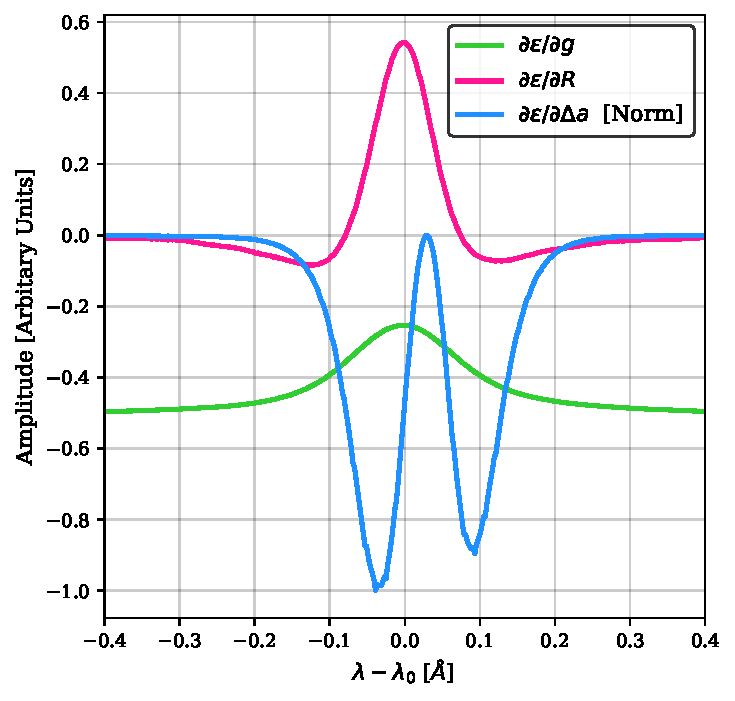
\includegraphics[width=\textwidth]{figures/EtalonPaper/Derivadas.pdf}
  \end{minipage}\hfill
  \begin{minipage}[c]{0.37\textwidth}
    \caption{
      Derivatives of the error metric as a function of wavelength. The derivative with respect to $\Delta a$ has been normalized in order to fit the three curves in the same plot. \label{fig_etalon_corr: Derivatives}} 
  \end{minipage}
\end{figure}


A few key aspects arise when analyzing the merit function and its applicability on real data. The first point to bear in mind is that the shape of the object, $O(\lambda)$, is not known a priory. Therefore, we needed to provide a guess for it. The method works by assuming that differences between the prediction and the observation are caused exclusively by the etalon defects or the gain. If the object used during the fitting process differs considerably from the real one, the prediction and observation will have differences that will erroneously be identified as etalon defects or gain variations. This is the main source of errors for the method when applied to real data. Two approaches can be followed in order to address this issue. The first one consists of assuming the solar atlas profile as the object. This is a good approximation, provided the data to which the algorithm is applied to lack information about solar structure, either because they are observations of long integration times of the quiet sun or produced by averaging several quiet sun observations (flat fields). If this condition cannot be met, this approach is not valid. The second approach involves deriving an approximated object from the data themselves by deconvolving the mean profile of the observation with the etalon's transmission profile. This approach can account for any difference the real object may have with the solar atlas and thus has a greater resemblance to the real object. Nevertheless, the process of deconvolving is prone to errors when the sampling is insufficient and can introduce additional noise into the problem. We have tested both approaches to compare their performances on different scenarios in order to assess when to use one or the other.

\begin{figure}
\centering
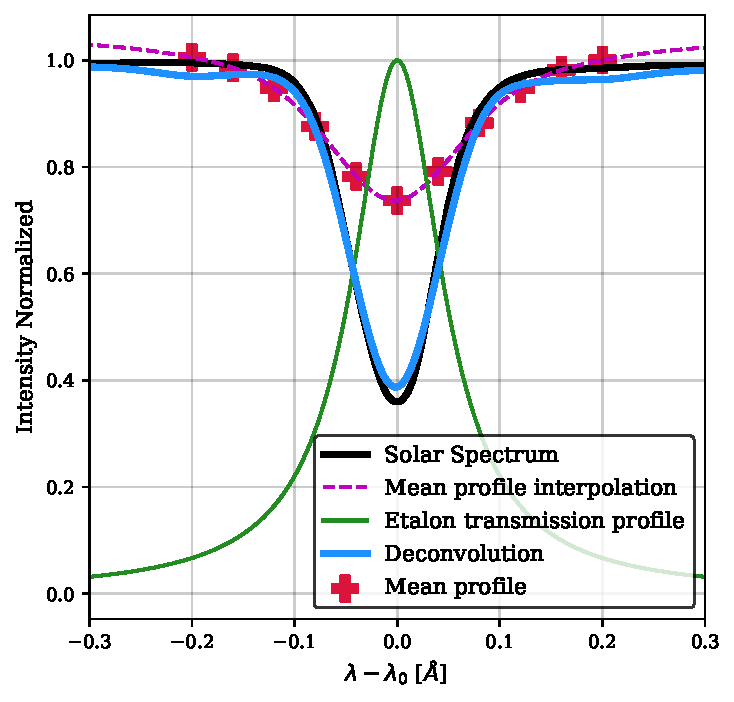
\includegraphics[width=\textwidth]{figures/EtalonPaper/Deconvolution.pdf}
\caption{Deconvolution of the object with a measurement of the Fe I spectral line using $N_\lambda = 9$. All points of the FoV have been used to compute the average profiles (blue crosses). The deconvolution (orange) is the result of deconvolving the mean profile interpolation (dashed line) with the displayed etalon transmission profile (red).\label{fig_etalon_corr:Deconvolution} }
\end{figure}

We employed Newton's method to minimize the merit function, Eq.~\eqref{eq_eta_corr: Merit Function}, as it has been proven to quickly converge (in five iterations or fewer, usually). The method begins by assuming an initial guess for the gain $g_j$ and $\Delta a_j$ parameters. Then, provided the initial guess is sufficiently close to the solution and that the merit function is continuous and differentiable, the gain $g_j$ and $\Delta a_j$ encoded in the vector, $\mathbf{x}_j$, can be updated iteratively at each iteration, $j$, as

\begin{equation}
\mathbf{x} _ {j + 1} = \mathbf{x} _ j - \mathcal{H} ^ {- 1} \mathcal{J} ^ T f(\mathbf{x}_j) \ , 
\end{equation}

where $\mathcal{H}$ and $\mathcal{J}$ are the Hessian and Jacobian matrices of the merit function $f$, respectively, calculated for $\mathbf{x}_j = [g_j,\Delta a_j]^T$, and $T$ stands for the transpose. Hence, the transmission profile of the etalon and its derivatives have to be computed for every wavelength and every pixel at each iteration. This can be computationally costly, especially when using imperfect telecentric configurations, where numerical integrals are involved. All derivatives needed for the algorithm are calculated analytically, except when simulating imperfect telecentrism. A detailed formulation of these derivatives is provided in the appendix.

Regarding the object $O(\lambda)$, if we assume it is given by the solar atlas, no additional computations are needed. However, when using the deconvolution approach, the object has to be calculated in each iteration. In this case, the algorithm works as follows: First, we compute the average profile across the whole FoV, and we force the continuum intensity to be the same on both sides of the spectral range to reduce the boundary effects of the deconvolution. This step is only necessary in case the spectral line is sampled in only a few positions, as is the case of the SO/PHI, IMaX, or TuMag instruments, where only a continuum point, either at the red or the blue side of the spectrum, is recorded. Both the object and transmission profile require a good spectral sampling to accurately compute the integrals of Eq.~\eqref{eq_eta_corr: Error metric}. Second, a cubic spline interpolation is applied to the generated average profile to artificially improve the spectral sampling, if necessary. Finally, the interpolated profile is then deconvolved by means of a Wiener filter with the etalon's transmission profile. The result of this deconvolution is the object, $O(\lambda)$, used in the minimization algorithm. The deconvolution of the object is done every time the etalon defects are updated in order to improve the resemblance of the deconvolved object to the real one. Figure \ref{fig_etalon_corr:Deconvolution} shows an example of this process in a simulated observation using nine scanned points and a collimated configuration. The deconvolution manages to reproduce the original signal, with only some minor differences in the line core and the beginning of the wings.

\subsection{\label{eta_corr_susec: results}Test scenarios and results}

The aim of the simulations carried out in this section was to characterize the role of the noise $\delta _ i ^ {\lambda_s}$, the spectral sampling, the selection of the object $O(\lambda)$, and the accuracy of the method for both the collimated and telecentric configurations. All simulations were run for different choices of the number of scanned wavelengths, ranging from $N_\lambda=5$ to $N_\lambda=21$. 

\subsubsection{Impact of the noise level}
We first assumed that the spectrum of the observed object is given by the solar atlas. This way, all errors in the derivation of the gain and etalon defects only come from the noise introduced into the measurement. We refer to this as the "ideal case." Since we were combining different measurements taken at different wavelengths, we considered a worst-case scenario and simulated three different signal-to-noise ratios: 100, 150, and 200. 

We restricted imperfections in the telecentrism to arise only for one scenario, S/N~$=200$, since simulating imperfections requires a high computational effort due to the lack of a theoretical expression for both the transmission profile and its derivatives. We also assumed that the degree of telecentrism ($0.3 ^\circ $) is known in this case.

\begin{figure}
    \centering
     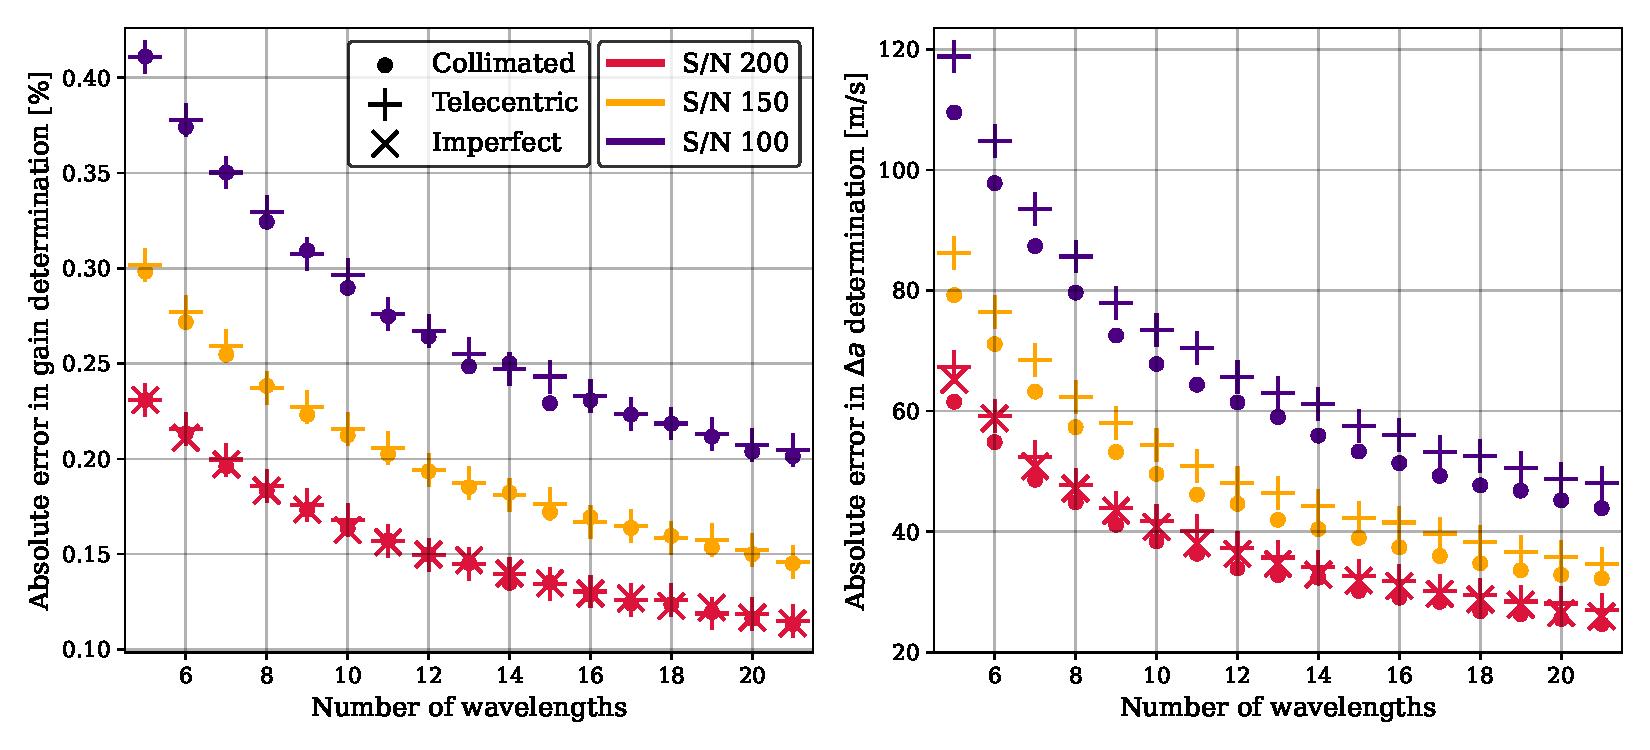
\includegraphics[width=\textwidth]{figures/EtalonPaper/SNR_plot_imperfect.pdf}
    \caption{Absolute errors of the gain (left) and etalon defect (right) derivations averaged over all the FoV. The number of wavelengths corresponds to the parameter $N_\lambda$ of wavelengths used to scan the profile.\label{fig_etalon_corr:SNR_both}}
\end{figure}

Figure \ref{fig_etalon_corr:SNR_both} shows the average absolute error in $g$ (left panel) and in $\Delta a$ (right panel) over the whole FoV as a function of the wavelength sampling, $N_\lambda$. The error in $g$ is expressed as a percentage of its real value. Errors in $\Delta a$ are given in meters per second since they are mostly responsible for shifting the profile. Errors in $\Delta a$ can be translated into velocity errors by computing the doppler velocity (Eq. \eqref{eq_spectro: Doppler}) associated to the spectral shift of the transmission ppeak produce by the error in $\Delta a$.
Figure \ref{fig_etalon_corr:SNR_both} shows the average absolute error in $g$ (left panel) and in $\Delta a$ (right panel) over the whole FoV as a function of the wavelength sampling, $N_\lambda$. The error in $g$ is expressed as a percentage of its real value. Errors in $\Delta a$ are given in meters per second since they are mostly responsible for shifting the profile. Errors in $\Delta a$ can be translated into velocity errors by computing the doppler velocity (Eq. \eqref{eq_spectro: Doppler}) associated to the spectral shift of the transmission ppeak produce by the error in $\Delta a$.

All the scenarios exhibit a similar behavior as far as their dependence on the spectral sampling is concerned, namely, the absolute errors decrease monotonically when the wavelength sampling increases. The reason for this is simply that a larger number of wavelength samples increases the amount of available information that the algorithm can use, thus making the fitting for $g$ and $\Delta a$ more precise. These results highlight the importance of properly sampling the targeted spectral line. A modest sampling of only $N_\lambda=5$ can produce errors as large as $120 \, {\rm ms^{-1}}$ in the worst-case scenario (S/N = 100). 

The noise level also plays an important role in the accuracy of the results. Scenarios with a lower S/N always have larger errors, for a given $N_\lambda$, in both the gain and $\Delta a $ computations. The difference in the performance of the algorithm due to the noise also changes with the spectral sampling; scenarios with a poor spectral sampling suffer from larger differences in the accuracy between the different S/N (50 ms$^{-1}$ for $N_\lambda$ = 5 between S/N = 200 and S/N = 100) than those with higher samplings (35 ms$^{-1}$ for $N_\lambda = 21$).

The optical configuration of the etalon has a very small impact on the accuracy of the algorithm. Results for the three setups are very similar, particularly in the gain calculation, for which the results are almost identical for all configurations. Retrieval of $\Delta a$ is slightly better for the collimated mount, though.

\begin{figure}
    \centering
    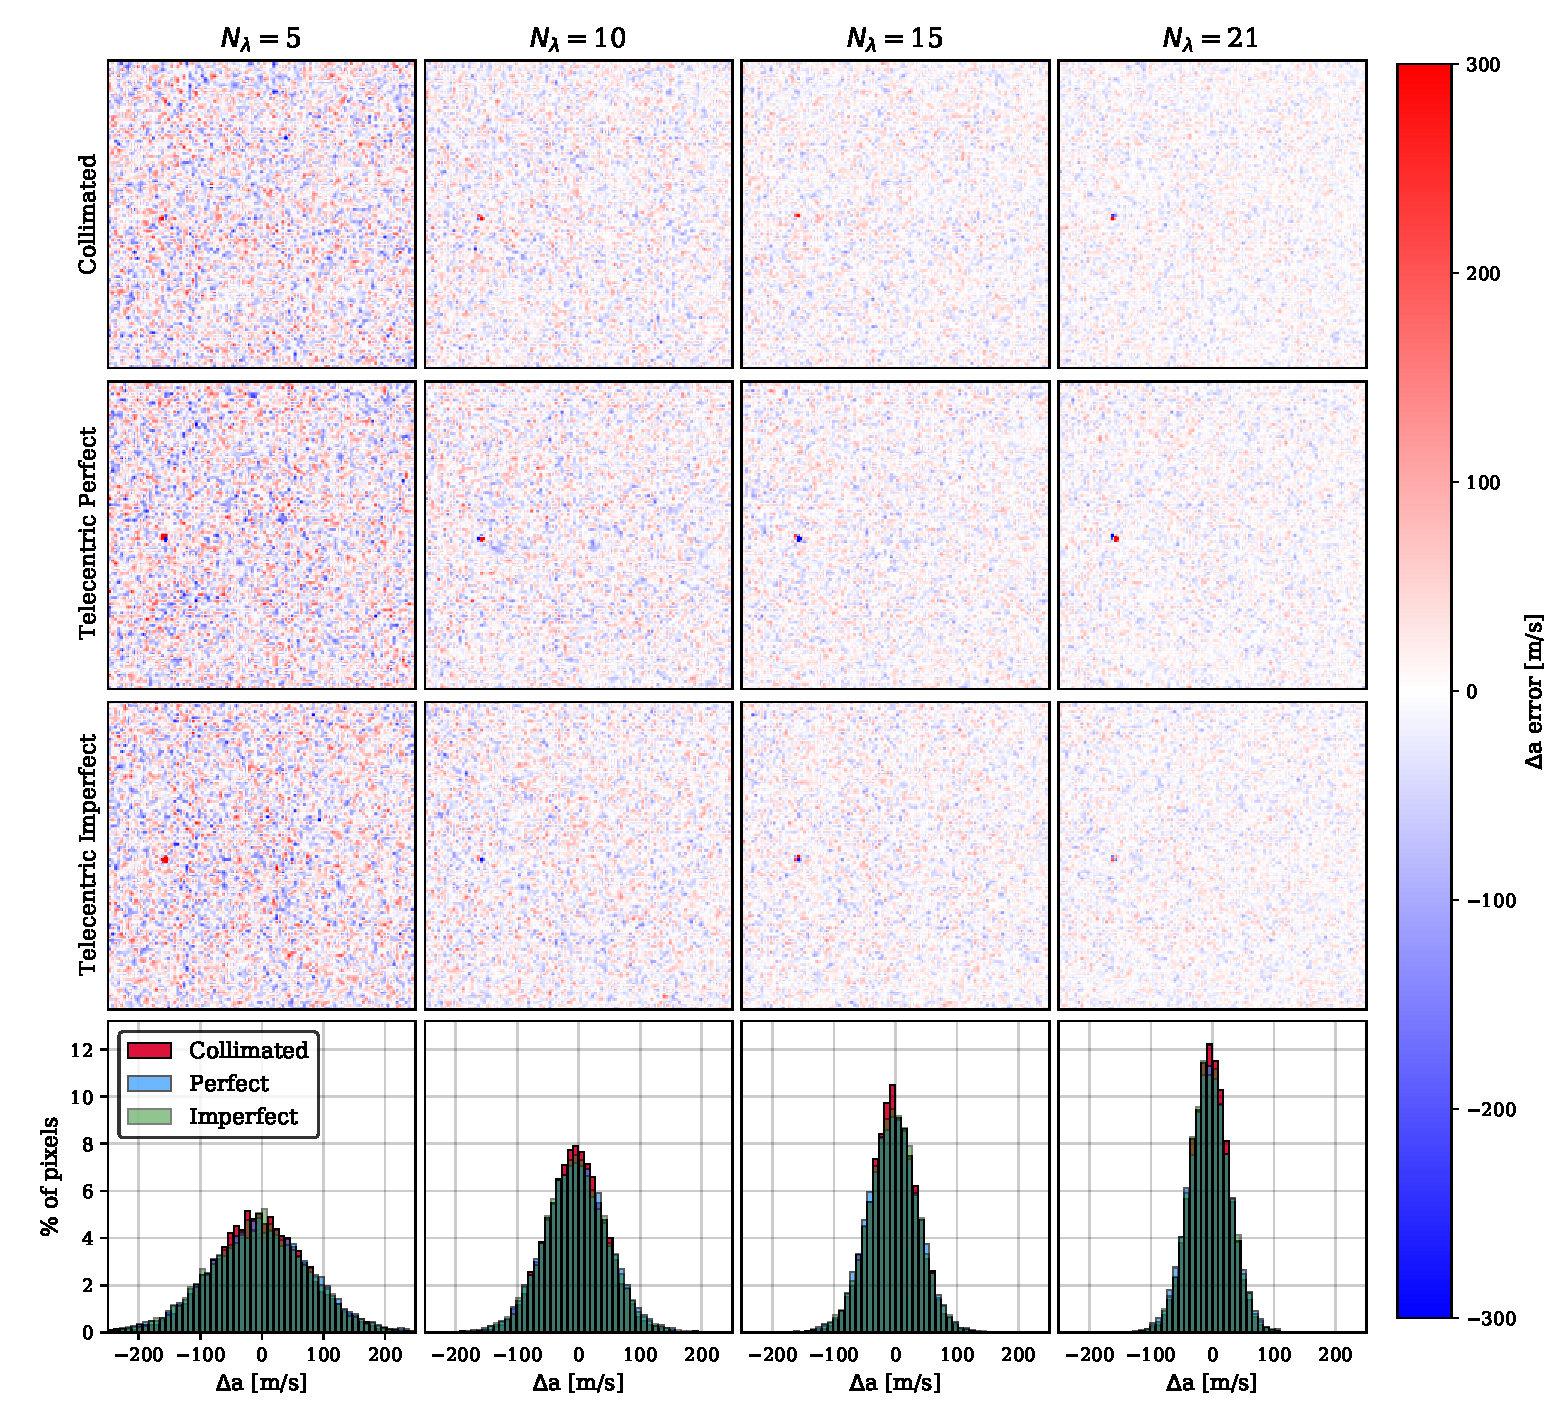
\includegraphics[width=\textwidth]{figures/EtalonPaper/Maps_Fov_Hist.pdf}
    \caption{Distribution of the errors in the $\Delta a$ computation for the three configurations (first three rows) and different spectral samplings (columns). In the bottom panels of each column, the error distribution for the corresponding spectral sampling is shown for the three configurations. }
   \label{fig_etalon_corr:FOV}
\end{figure}

Figure \ref{fig_etalon_corr:FOV} shows the spatial distribution of the errors in the retrieval of $\Delta a$ for different choices of $N_\lambda$. There are no signs of a radial distribution in the maps shown in the figure, contrary to the actual distribution of the $\Delta a$ parameter, as shown in Fig.~\ref{fig_etalon_corr: Inputs}, bottom panel. This means that the precision of the method is similar no matter the amplitude of the defects, that is, we achieve the same accuracy in the retrieval of defects associated with shifts of 3 pm ($\sim$ 1450 ms$^{-1}$, near the corners of our FoV), which correspond to cavity errors of around 1.5 nm or incidence angles of approximately 0.4 degrees, and in the retrieval of regions where no defect is present (radius of 20 pixels from the center of the FoV approximately). Instead of a radial distribution, the errors follow a Gaussian-like distribution (shown at the bottom panels in \ref{fig_etalon_corr:FOV}) similar to the one followed by the noise contribution.

The standard deviation of the errors for both the gain and $\Delta a$ computations are also reduced with an increase in spectral sampling. The last row of Fig. \ref{fig_etalon_corr:FOV} displays the error distributions in the calculation of  $\Delta a$ for the three optical configurations and different spectral samplings. These results illustrate how the three configurations yield practically identical results and how the distribution narrows as $N_\lambda$ increases, thereby improving the results. Specifically, the standard deviation decreases from 50 ms$^{-1}$ for $N_\lambda = 5$ to 20 ms$^{-1}$ for $N_\lambda = 21$. In the case of the gain determination, the standard deviation ranges between 0.2 \% and 0.1\% for the scenarios with the poorest and highest spectral sampling, respectively.

\subsubsection{\label{sect: fitting_deconv}Impact of the object approximation}

To infer the error of the algorithm when the object is unknown, we compared the performance of the ideal case, that is, when the object used to generate the observations is known, with the one achieved when deconvolving the object from the data. Only the collimated setup was simulated in order to focus exclusively on the errors introduced by the deconvolution. The data has been degraded by Gaussian noise with an S/N = 200 in both scenarios. 

\begin{figure}
    \centering
     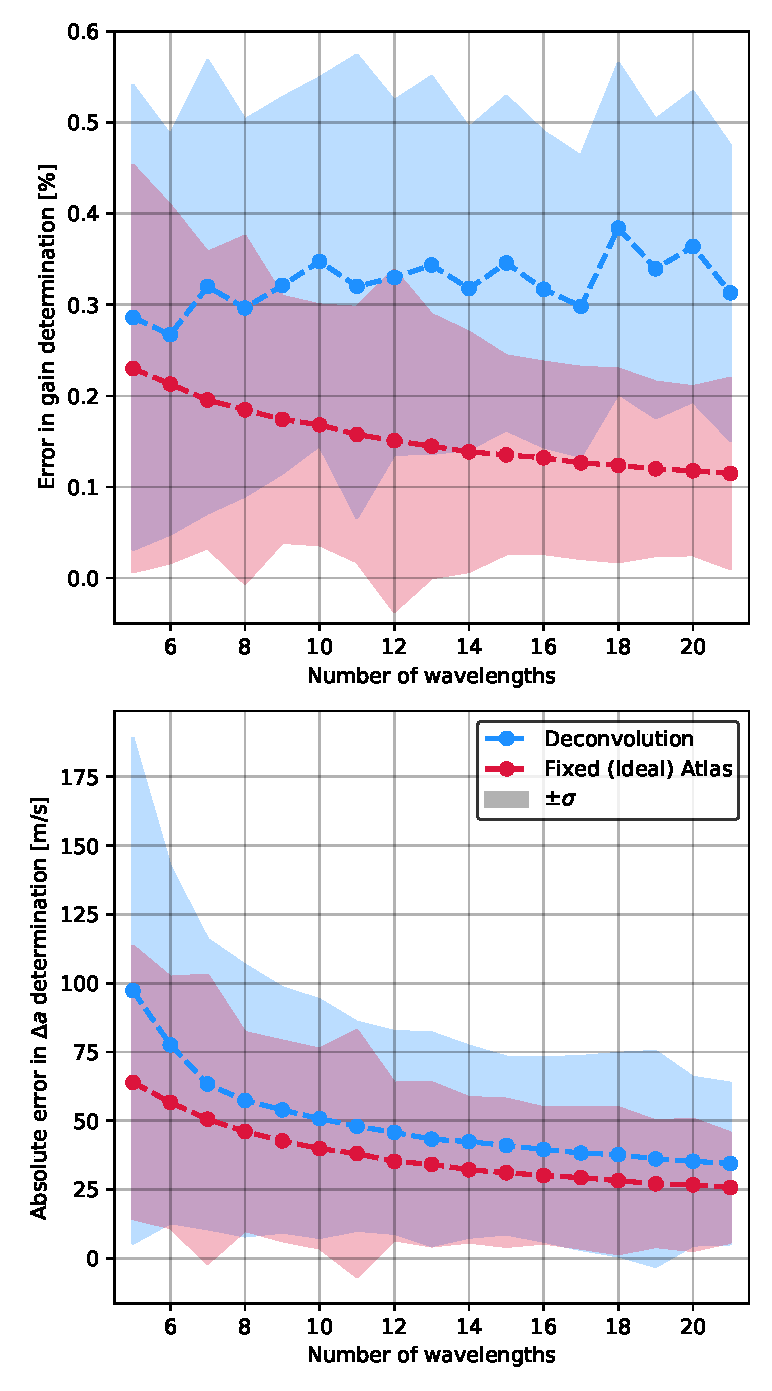
\includegraphics[width=\textwidth]{figures/EtalonPaper/Deconvolution_results.pdf}
    \caption{Errors in gain determination and etalon properties averaged over all the FoV with a signal-to-noise ratio of 200 and a collimated configuration.}
    \label{fig_etalon_corr:Deconvolution-results}
\end{figure}

Figure \ref{fig_etalon_corr:Deconvolution-results} shows the results for the two approaches. Interestingly, the error in the gain for the deconvolution approach does not decrease with a larger number of wavelengths, unlike the ideal case. Nevertheless, the average error of the calculation is below 0.4~\%, with a dispersion (1 $\sigma$) of $\pm$ 0.3~\%. The deconvolution approach is prone to higher errors when deriving the gain due to the normalization of the profiles. The reason for this is two-fold. first, if the continuum is far enough from the spectral line, the normalization is strictly the integral over the transmission profile because the object is flat along the integration interval. However, this is not strictly true since the wings of the transmission profile can reach the spectral line (see Fig.~\ref{fig_etalon_corr: Prof-Measure}), hence modifying the normalization of the profile when the object changes at each iteration. Second, should the continuum intensity of the derived object vary with respect to its real value due to the deconvolution process (e.g., due to boundary effects), there will be a shift in the intensity of the whole profile induced by the normalization process. These two effects seem to dominate the accuracy on the gain determination, regardless of the chosen sampling.

For $\Delta a$, the performance of the method is slightly worse than for the ideal case when using the deconvolution approach. Unlike the gain determination, errors in the $\Delta a$ derivation show a strong dependence on the spectral sampling. Differences between both approaches range from $10$~ms$^{-1}$ to $40$~ms$^{-1}$ and increase with decreasing $N_\lambda$. The sensitivity with $N_\lambda$ is especially high up to $N_\lambda = 8$. A modest increase of $N_\lambda$ from five to six improves the determination of $\Delta a \sim$ 20 ms$^{-1}$, whereas at better spectral samplings, the difference between each simulation decreases more slowly, without any relevant improvement as the sampling increases. In any case, differences are all well within $\pm 1\sigma$.

\subsubsection{The crossover case}

The fact that the sensitivity of the model to the gain and to the $\Delta a$ parameters are different guarantees (to some extent) that the parameters can be separated from each other. The treatment of the problem is very different between etalon configurations, and therefore full knowledge of the setup is critical. However, this is not always feasible due to the unavoidable presence of errors, misalignment, and imperfections on the instrument. Approximations to describe the optical setup are also common in the pipeline of an FPI instrument because they reduce computational efforts. For instance, telecentric mounts are usually simplified as collimated setups, as the f-numbers employed in solar instruments are usually very large. Imperfections of telecentrism are commonly neglected, too. In this section, we analyze the impact of assuming an incorrect etalon mounting. To do so, we repeated the previous exercise, starting from a perfect and imperfect telecentric configuration but assuming that the transmission profile shape corresponds to a collimated one.    

\begin{figure}
    \begin{minipage}[c]{0.6\textwidth}
      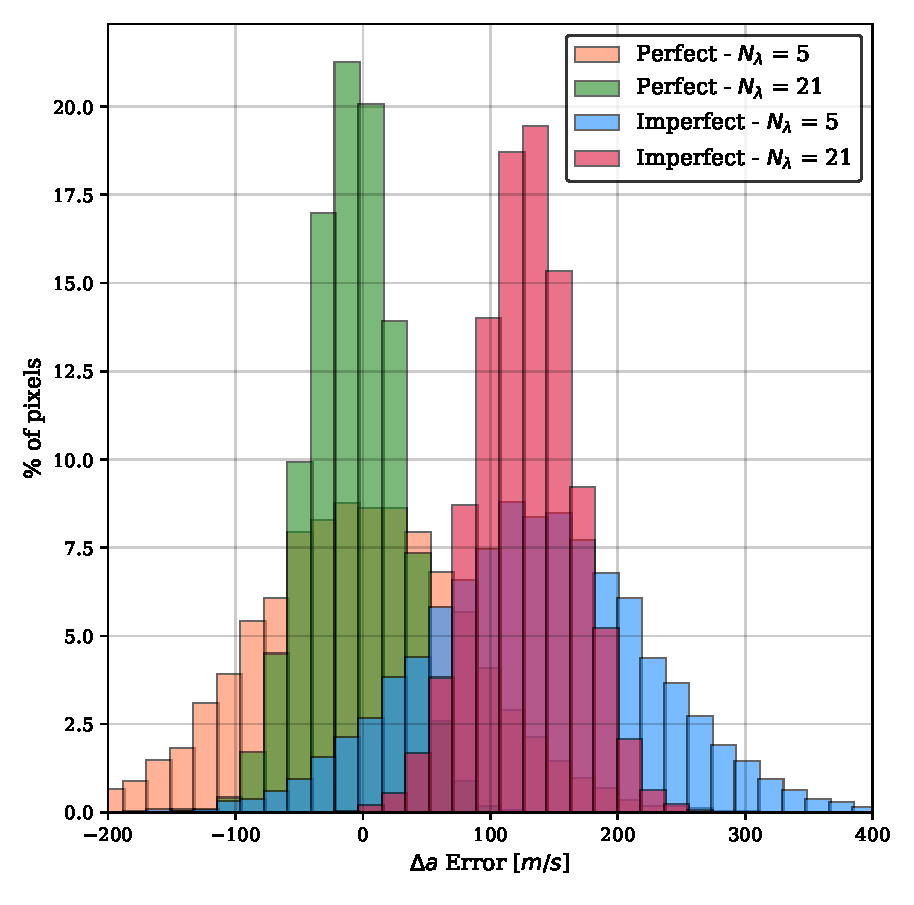
\includegraphics[width=\textwidth]{figures/EtalonPaper/histograms.pdf}
    \end{minipage}\hfill
    \begin{minipage}[c]{0.37\textwidth}
      \caption{
        Distribution of the errors in the determination of $\Delta a$ for the crossover scenarios (different configuration in the observation generation and minimization algorithm) for both perfect and imperfect configurations. Only results for the two extreme spectral samplings ($N_ \lambda = 5$ and $N_\lambda = 21$) are shown.
      } \label{fig_etalon_corr:Crossover_histograms}
    \end{minipage}
  \end{figure}

In this exercise, we assumed that we have an instrument with an FPI in a telecentric mount, as in the previous sections, in both perfect and imperfect configurations and an S/N~$=200$. We also considered that the object is given by the spectral solar atlas. The shift of the perfect telecentric transmission profile with respect to the collimated one was corrected using Eq.52 from \cite{franI} to avoid the emergence of spurious velocity signals. Imperfections in the telecentrism shift the profile more. This additional displacement was left uncorrected intentionally so we could study its effects.

Figure \ref{fig_etalon_corr:Crossover_histograms} shows the error distributions for $\Delta a$ when the model assumes a collimated configuration for $N_\lambda=5$ and $N_\lambda=21$ and for both perfect and imperfect configurations. The amplitude and dispersion of the error distributions are very similar for the two mounts and are comparable to the results obtained in the ideal case (Fig.~\ref{fig_etalon_corr:FOV}, bottom panel). The main difference between the perfect and imperfect scenarios is a shift of $130$ ms$^{-1}$ for the reason mentioned above. We note that this shift can easily be accounted for since it is a known and measurable effect. 

The similarity in the error distributions for the calculation of $\Delta a$ in the two scenarios demonstrates that the error incurred when assuming a collimated etalon does not significantly impact the determination of the cavity maps of the etalon. This is because changes in $\Delta a$ mostly induce a shift of the transmission peak by an equal amount in both cases.

\begin{figure}
  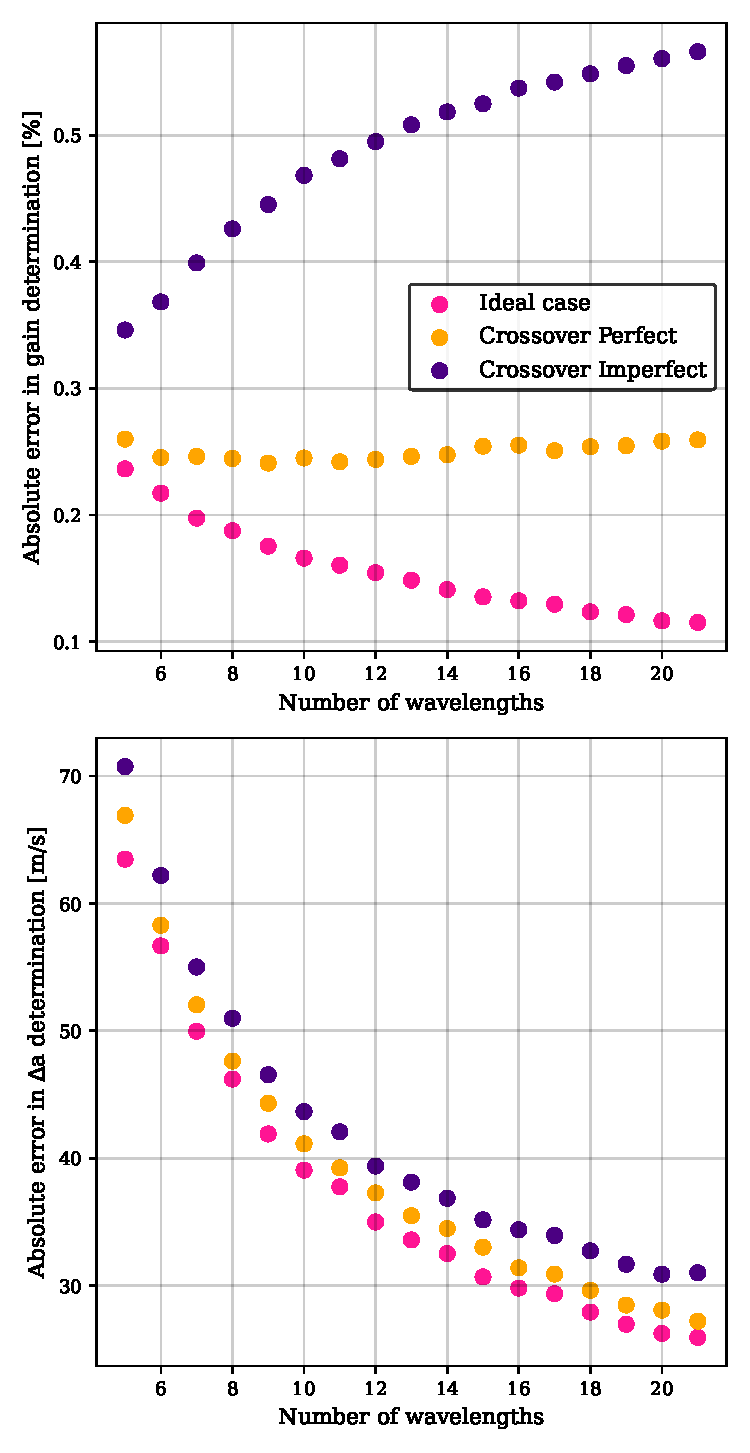
\includegraphics[width=\textwidth]{figures/EtalonPaper/means.pdf}
  \caption{Average errors of the gain (left) and etalon defect (right) calculations over all the FoV for the two crossover cases and the standard case (also shown in Fig.~ \ref{fig_etalon_corr:SNR_both} as the collimated case with S/N = 200) for reference. All $\Delta a$ errors have been computed by correcting differential offsets of the transmission profile between the different mounts.\label{fig_etalon_corr:crossover}}  
\end{figure}

We note, however, that the amplitude, width, and shape of the transmission profile differ significantly between the telecentric and collimated configurations, leading to an expected higher error in gain calculation. Figure \ref{fig_etalon_corr:crossover} shows the absolute errors in gain and $\Delta a$ calculations for both crossover scenarios and the ideal case after correcting the wavelength shift between the different mounts. For $\Delta a$, the performance of the method is very similar in the three setups, as also observed earlier. This behavior is nevertheless anticipated since the properties selected for simulating the imperfect etalon were chosen to mirror those of the SO-PHI etalon, which were adjusted to closely resemble the behavior of a collimated etalon to the greatest extent possible.

The differences are larger for the gain determination. Not only are the errors higher in the crossover cases, but the trend is entirely different. Instead of decreasing when increasing the number of wavelengths, gain errors remain the same for the perfect case and increase with the number of samples for the imperfect case. Similar to the deconvolution case (Fig.~\ref{fig_etalon_corr:Deconvolution-results}), the difference between transmission profiles introduces an error in the normalization process that systematically affects the rest of the measurements. This effect becomes more pronounced as the number of wavelengths increases, given that this error is introduced more frequently, and it is even more prominent in the imperfect case, as not only are the profiles different in this scenario, but they are also asymmetric. This asymmetry results in an imbalance in the measurement of the profile, as one wing of the spectral line has a higher transmissivity and is observed with greater intensity than the other.

Our results suggest that assuming an etalon in a collimated configuration for instruments with telecentric mounts can be a good first-order approximation for cavity map calculations, provided that the level of asymmetry of the transmission profile is known. However, achieving an accurate knowledge of the degree of telecentrism is often challenging in real instruments, as it usually varies across the FoV. Meanwhile, the results highlight that this approximation leads to a considerable increase in the error in the gain determination, which increases when increasing the spectral sampling. This contrasts with the standard philosophy of solar instrumentation, which requires a high number of points to better scan the spectral line.

\subsubsection{Real data}

While simulated tests are crucial for understanding the algorithm's behavior as a function of the different parameters of the problem, tests with real data are required to validate the effectiveness of the method. In this section, we evaluate the results obtained by the algorithm when implemented on observations acquired using the High-Resolution Telescope (HRT) of the SO/PHI instrument. 

The observation we used corresponds to a flat-field observation employing six points to scan the 6173 \r{A} line (five along the spectral line and an additional continuum measurement) conducted on March 9, 2022. The FPI aboard SO/PHI is illuminated in a telecentric mount, with an expected degree of telecentrism of about $0.3^\circ$. The tests conducted with this dataset have the same procedure as the ones employed for simulated data, that is, we only fit the gain and $\Delta a$ parameters, and we employed the deconvolution approach (Sect. \ref{sect: fitting_deconv}).

\begin{figure}
  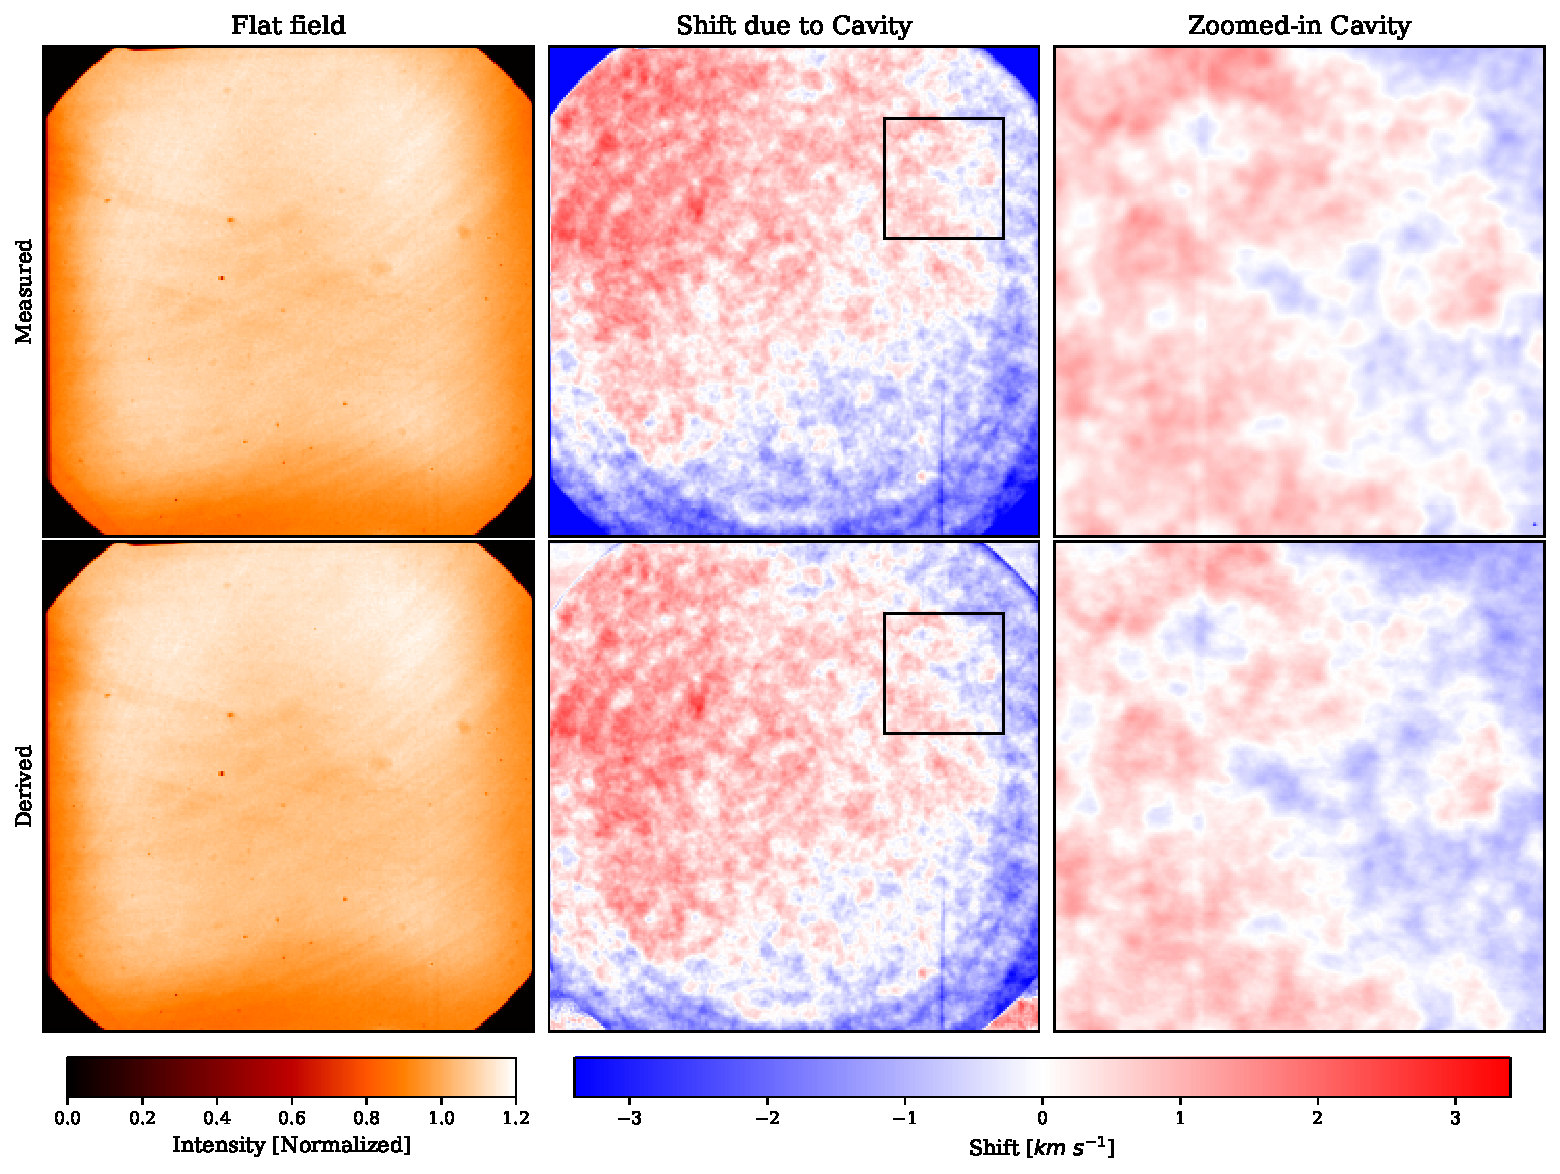
\includegraphics[width=\textwidth]{figures/EtalonPaper/Comparison_HRT.pdf}
  \caption{Comparison between the observed flat-field and cavity map (top row, left and center columns, respectively) and the derived flat-field (gain) and cavity map ($\Delta a$; bottom row, left and center columns, respectively). The right column in both rows showcases a zoomed-in region of each cavity map. The area corresponding to the zoomed-in region is indicated with a black square in the full cavity map to its left. The properties used to simulate SO/PHI's etalon are $R = 0.925$, $n=2.29$, $d = 251.63\ \mu m$, $f\# = 60$, $\Theta = 0.23 ^{\circ}$.\label{fig_etalon_corr:HRT}}  
\end{figure}

Figure \ref{fig_etalon_corr:HRT} shows the results obtained when applying the algorithm to HRT-SO/PHI data. The top row shows, from left to right, the observed flat at the continuum, the cavity map measured under laboratory conditions (on ground), and a selected region of the cavity map. In the bottom row, the same cases are shown but for the results inferred by the algorithm. That is, the flat-field (i.e., the gain) and the cavity map (i.e., $\Delta a$).

The results obtained for the cavity map closely resemble the laboratory measurements. The overall structure is preserved, maintaining the gradient from the upper left to the lower right. Similar structures are also discernible, such as the vertical line in the lower-right corner and the ring-like patterns evident in the lower section of the image. However, closer scrutiny of the observed structures revealed some differences. This deviation between results and measurements is expected, considering that the experiment conducted here represents a first-order approximation to assess the algorithm's capability to generate coherent results. Several factors contribute to these differences. Firstly, the spatial resolution of the cavity measured on ground is lower. Secondly, the degree of telecentrism has a predicted variation of $0.23^\circ$ across the FoV. Thirdly, we expected an error for the six-point scan, employing the deconvolution strategy, as large as a hundred meters per second.

Concerning the results for the gain determination, the comparison depicted in Fig.~ \ref{fig_etalon_corr:HRT} suggests that pixel-to-pixel gain variations can also be determined accurately with our method, as both small-scale and large-scale variations are reproduced with detail. 

\begin{figure}
  \centering
  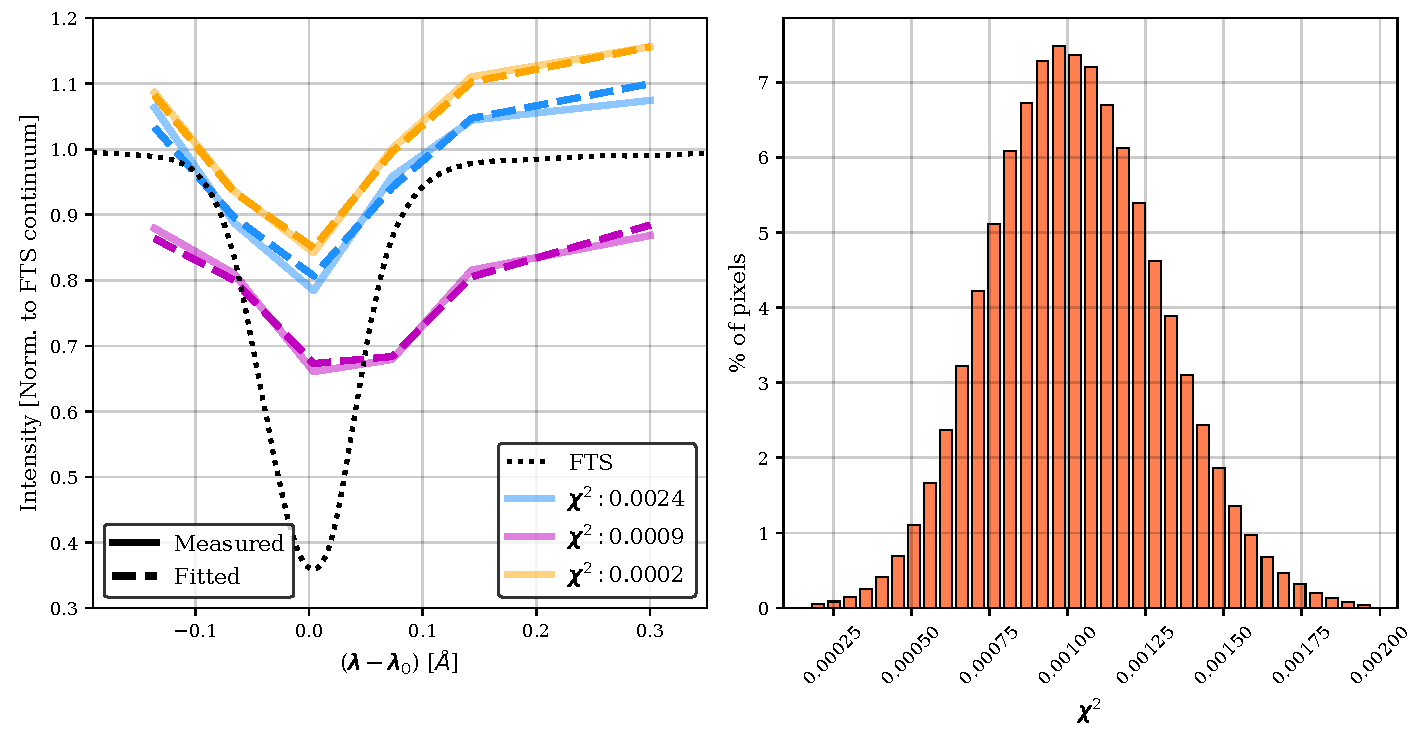
\includegraphics[width=\textwidth]{figures/EtalonPaper/fitting_chisq_hor.pdf}
  \caption{Comparison between the measured (solid lines) and fitted profiles (dashed lines) for three pixels, each representing varying degrees of accuracy (top panel). The FTS is shown as a reference. The bottom panel displays the distribution of $\chi^2$ values for all pixels. Among the three selected cases, one demonstrates an average fit (depicted in pink, with $\chi^2$ close to the mean value), while the other two correspond with extreme cases—one with a notably good fit and the other with a poor fit (depicted in yellow and blue, respectively). The value for $\chi ^2$ has been computed employing equation \eqref{eq_eta_corr: Merit Function}\label{fig_etalon_corr: xisq_hrt}}  
\end{figure}

A more quantitative analysis of the results is depicted in Fig.~\ref{fig_etalon_corr: xisq_hrt}. The upper panel shows a comparison between the fitted and observed profiles for three distinct cases with varying degrees of precision, while the bottom panel shows the distribution of $\chi^2$ for all pixels. In the worst-case scenario, small differences between the real profile and the fit can be seen in both the line wing and the line core. In any other case, the fittings are rather satisfactory.


\subsection{Algorithm applied at the Sunspot}

.

\section{Conclusions.}

In this chapter we have highlighted the relevance of carefully addressing the data reduction of etalon-based instruments, specifically those with the FPI in telecentric setups. Equipped with the analytical modelling of the FPIs, we have been able to address the impact of the etalon defects on the observations through a series of simulations. We have quantified the error commited in the computations of LOS velocities and magentic fields when the cavity errors are (only) partially corrected through the simulation of an observation of a Sunspot. Additionally, we have provided a new strategy for the data correction of etalon-based spectrometers that separates the effects of the FPIs on the flat-fields from other effects in order to improve the flat-field correction. Lastly, we have tested the performance of this new method on a series of simulated observations and real data to verify its applicability. 

The simulation of the sunspot observation in section \ref{sect: Mancha_obs} demonstrates the significant impact of improperly corrected cavity errors on the physical measurements. The discussion is centered around the flat-fielding procedure, which presents one of the main challenges in these setups, as cavity errors also affect flat-field observations. We show that these flat-fields alter and distort the observed spectral profiles when applied. The correlation between the structures found in the velocity calculation errors after flat-field correction and those of the cavity map suggests that the flat-fielding has not (fully) corrected these errors. In the penumbra, errors can reach up to 400 ms$^{-1}$ for both flat-fielding approaches, which would invalidate any measurements, as penumbral flows are of similar magnitudes.

Furthermore, we found that the shape of the transmission profile affects the measurements, with velocities derived using an asymmetrical transmission profile differing from those obtained with a symmetrical one. This, combined with the distinct behavior of the umbra compared to the rest of the field of view (FoV), implies that these measurements are sensitive to both the shape of the transmission profile and the spectral profile of the object.

Similar effects are observed in the magnetic field calculations, where the error structures correspond to those of the cavity map. However, in the case of magnetic fields, this effect is less significant, as the error values are small relative to the observed values (3 G of error in a 100 G field).

These results motivate the pursuit of methods to account for and correct these effects. One such method is the algorithm we developed to disentangle the FPI-based spurious effects on the flat-fields from those of other origins. The method, presented in Section \ref{sect: etalon_corr_fitting}, is capable of extracting the cavity map from the observations by employing the analytical modeling of the FPIs in different configurations.

We evaluated the performance of the algorithm through a series of simulated tests designed to assess various key aspects of its applicability to real data. In the first place, the performance of the algorithm was tested as a function of the S/N of the observations, the spectral sampling, and the configuration of the etalon, assuming the spectrum of the object is known. We also studied the possibility of deriving the observed object from the data through a deconvolution process. We tested the performance of this approach as a function of the spectral sampling. Finally, we simulated a scenario in which the etalon configuration was different from the real one. The aim of these tests was to assess the impact of neglecting some properties of the etalon, such as the asymmetries in telecentric imperfect scenarios.

The algorithm has shown a high sensitivity to the noise level of the data. Nonetheless, the worst-case scenario considered in this work corresponds to much worse performances than current instruments can achieve in terms of S/N, and the errors are still within the necessary limits. In addition, the performance of the algorithm is the same for regions of the FoV where the etalon properties are far from their nominal values and regions where there is no deviation of the etalon properties. 

Results for the three different optical configurations of the etalon are very similar. The telecentric configuration showed a worse performance than the collimated one in terms of cavity map retrieval. The loss of precision is nonetheless very small, below $\sim 5$~ms$^{-1}$ in most cases. 

The deconvolution of the object during the calculations was shown to yield a performance close to the ideal case in terms of cavity map determination. The performance when computing the gain showed a different behavior, although the average error never exceeds 0.4\%. Concerning the dependence on the spectral sampling, the results show that with a scanning of at least six points, the additional error of deconvolving the object will not be larger than 25~ms$^{-1}$. Overall, we estimated a total error smaller than 100~ms$^{-1}$ for the worst-case scenario, where only five wavelengths are used to scan the line using the deconvolution approach for an S/N of 200.

In real instruments, light travels through different optical elements before reaching the etalon. Along this light path, the observed object might be modified in such a way that it no longer resembles a fixed reference. It is in fact very difficult to assess the error associated with this assumption (i.e., assuming that the object reaching the etalon is that of the FTS atlas profile) since these deviations cannot be measured. By deriving the object from the data, we expect additional errors due to the deconvolution process of around 10~ms$^{-1}$, which we expect to be smaller than the ones produced by selecting a fixed object that differs considerably from the real one. Additionally, the deconvolution of the object allowed us to apply the algorithm to data where a solar structure is partly present.

Knowledge of the exact shape of the transmission profile has proven to be relevant to ensuring the accuracy of the algorithm. The results obtained for the crossover scenario have demonstrated that approximating the FPI's transmission profile by another can serve as a first-order approximation. However, the determination of the gain has proven to be much more sensitive to changes in the transmission profile. The errors observed in the crossover scenario are higher overall than those of the ideal case. In addition, the unaccounted asymmetries of the imperfect configuration paradoxically increase the error when improving the spectral sampling.

The results obtained when applying the algorithm to real observations taken with SO/PHI reinforce the validity of the algorithm. Indeed, we have been able to extract the contribution of the cavity map from the flat-field observations. Comparison of the derived cavity map with lab measurements suggests that the algorithm can successfully extract the cavity map from the flat-field observations. In future works, we aim to allow the algorithm to modify the angle of incidence across the FoV and validate the results by implementing them in the SO/PHI pipeline.


